\documentclass[11pt,letterpaper]{article}

\usepackage{cvpr}
\usepackage{times}
\usepackage{epsfig}
\usepackage{graphicx}
\usepackage{amsmath}
\usepackage{amssymb}

\usepackage{authblk}
\usepackage{bm}
\usepackage{mathtools}
\usepackage{mdframed}%
\usepackage[ruled]{algorithm2e}
\usepackage{enumitem}
\usepackage{lipsum}%
\usepackage{url}%
\usepackage{multicol}
\usepackage[bottom]{footmisc}

\usepackage[pagebackref=true,breaklinks=true,letterpaper=true,bookmarks=false,colorlinks]{hyperref}
% color for refs (equations, acros)
\hypersetup{linkcolor=blue}

\cvprfinalcopy

\def\httilde{\mbox{\tt\raisebox{-.5ex}{\symbol{126}}}}

\ifcvprfinal\pagestyle{empty}\fi

\DeclareMathAlphabet\mathbfcal{OMS}{cmsy}{b}{n}
\DeclareMathOperator*{\argmin}{arg\,min}

\SetKwInput{kwObjective}{Objective}
\SetKwInput{kwAlgorithm}{Algorithm}

\numberwithin{equation}{section}

\graphicspath{{../}}

\usepackage{acronym}

\AtBeginEnvironment{acronym}{
	\renewcommand*{\aclabelfont}[1]{\acsfont{\color{blue}#1}}}
	
\usepackage{subfigure}

\begin{document}

\title{Comparative Analysis of Two-View and Three-View Pose Estimation Algorithms for Image-Based 3D Reconstruction: Fundamental Matrix vs Trifocal Tensor \\ IACV 2023-2024 Project}

\author[1]{Giovanni Versiglioni}
\author[2]{Luca Magri}
\author[2]{Federica Arrigoni}
\author[2]{Vincenzo Caglioti}
\affil[1]{\textbf{[Student]} giovanni.versiglioni@mail.polimi.it}
\affil[2]{\textbf{[Supervisors]} luca.magri@polimi.it, federica.arrigoni@polimi.it, vincenzo.caglioti@polimi.it}

\maketitle

\begin{abstract}
	Image-based 3D reconstruction is crucial in areas like computer vision and augmented reality. Traditionally, most reconstruction algorithms have focused on using two images at a time. However, using three images together can apply stricter geometric rules, potentially improving accuracy. The trifocal tensor is generally favoured over the fundamental matrix when working with three views. This research project compares existing methods for two-view and three-view pose estimation, challengeing this preference by thoroughly investigating and comparing the performance of the trifocal tensor against the fundamental matrix.\\
	
	\textbf{Keywords} Multiple-View Geometry, Pose Estimation, Fundamental Matrix, Trifocal Tensor
\end{abstract}

\begin{multicols}{2}
\tableofcontents
\end{multicols}

\pagebreak

\listoffigures

\vspace{10mm}

\listoftables

\vspace{10mm}

\listofalgorithms

\pagebreak

\section*{List of Acronyms}
\begin{acronym}
 \acro{FM}{Fundamental Matrix}
 \acro{TFT}{Trifocal Tensor}
 \acro{L-FM}{Linear Fundamental Matrix Estimation}
 \acro{O-FM}{Optimized Fundamental Matrix Estimation}
 \acro{L-TFT}{Linear Trifocal Tensor Estimation}
 \acro{R-TFT}{Ressl Trifocal Tensor Estimation}
 \acro{N-TFT}{Nordberg Trifocal Tensor Estimation}
 \acro{FP-TFT}{Faugeras-Papadopoulo Trifocal Tensor Estimation}
 \acro{PH-TFT}{Ponce-Hebert Trifocal Tensor Estimation}
 \acro{GH}{Gauss-Helmert Optimization}
 \acro{LM}{Levenberg-Marquardt Optimization}
 \acro{DLT}{Direct Linear Transformation}
 \acro{BA}{Bundle Adjustment}
\end{acronym}

\pagebreak

\section{Introduction}\label{sec:intro}
Since the beginning of computer vision, cameras and images have been key areas of study. Central to this field are challenging tasks like figuring out positions and reconstructing 2D or 3D scenes. These tasks rely on understanding how points in space relate to their images, following the principles of perspective projection in pinhole cameras. This knowledge allows us to triangulate points in space from their projections in images.\\

Within this framework, the fundamental matrix is a key algebraic tool that captures the relationship between matching points in images. It helps us understand the relative positions and orientations of two camera views, which is crucial for many computer vision applications. Extending this to three views introduces the trifocal tensor, a mathematical construct that represents the relationships among three corresponding image points, known as trilinearities. While it's theoretically possible to create a multi-view matrix for any number of views, practical applications usually focus on pairs or triplets of views. As a result, most multi-view structure-from-motion techniques start with pairs or triplets of images for practical use.\\

Traditionally, the trifocal tensor is favoured over the fundamental matrix when working with three views. This work challenges this preference by thoroughly investigating and comparing the performance of the trifocal tensor against the fundamental matrix.\\

\subsection{Outline}

In Sections (\ref{sec:fm}) and (\ref{sec:tft}) we thoroughly define and explain the fundamental matrix and the trifocal tensor, respectively. Then, in Section (\ref{sec:estimation}) we present the methods used to determine camera poses, either using the fundamental matrix or the trifocal tensor. The performances of both are compared with empirical findings in Section (\ref{sec:experiments}). These results are analyzed in Section (\ref{sec:conclusions}), leading us to conclude that while the trifocal tensor has certain advantages, they are not significant enough to definitively consider it superior to the fundamental matrix.

\subsection{Notation}
In this paper, we adopt specific notation conventions: vectors are denoted by lowercase (\( v \)), matrices by uppercase (\( M \)), tensors by calligraphic bold uppercase (\( \mathbfcal{T} \)), and tensors' correlation slices (\ie, matrices) by bold uppercase (\( \bm{T}_i \)).\\

The \( 3 \times 3 \) matrix representation of the cross product with a 3-vector $v$ is indicated by \( [v]_{\times}w \), \ie, \( [v]_{\times}w = v \times w \), where \( w \) represents any given vector.\\

The \( L^2 \) norm of a vector \( v \) is denoted as \( \Vert v \Vert \), while for matrices or tensors, it represents the \( L^2 \) norm of the vector constructed from their coefficients. The Frobenius norm of a matrix \( M \) is denoted as \( \Vert M \Vert \), while for a tensor \( \mathbfcal{T} \), it signifies the square root of the sum of squares of all its elements, denoted as \( \Vert \mathbfcal{T} \Vert \coloneqq \sqrt{\sum_{i,j,k} (\bm{T}_{i}^{jk})^2} \).\\

Additionally, \( \vert M \vert \) refers to the determinant of matrix \( M \).

\section{The Fundamental Matrix}\label{sec:fm}
In this section, we begin by defining the fundamental matrix. Next, we outline numerical methods for estimating the fundamental matrix using point correspondences between two images. We start by using linear equations from epipolar constraints to build a basic framework. Then, we delve into \ac{GH} \cite{12-gauss-helmert} to improve precision and robustness in our analysis. A similar approach will be carried out for the trifocal tensor later on (Section \ref{sec:tft}).

\subsection{Definition}
The \ac{FM} is defined by the equation
\begin{equation}
	x'^\top Fx = 0
	\label{eq:fmDef}
\end{equation}

for any pair of matching points \( x \leftrightarrow x' \) in two images. 

\subsection{Linear Computation}
Given sufficiently many point matches (\ie, at least 7), Equation (\ref{eq:fmDef}) can be used to compute the unknown matrix \( F \). In particular, each point match gives rise to one linear equation in the unknown entries of \( F \). Specifically, the equation corresponding to a pair of points \( (x, y, 1) \) and \( (x', y', 1) \) is
\begin{equation}
	x'xf_{11} + x'yf_{12} + x'f_{13} + y'xf_{21} + y'yf_{22} + y'f_{23} + xf_{31} + yf_{32} + f_{33} = 0.
\end{equation}

From a set of \( n \) point matches, we derive the set of linear equations

\begin{equation}
	Af = 
	\begin{bmatrix}
	x_1'x_1 & x_1'y_1 & x_1' & y_1'x_1 & y_1'y_1 & y_1' & x_1 & y_1 & 1\\
	\vdots & \vdots & \vdots & \vdots & \vdots & \vdots & \vdots & \vdots & \vdots\\
	x_n'x_n & x_n'y_n & x_n' & y_n'x_n & y_n'y_n & y_n' & x_n & y_n & 1
	\end{bmatrix}
	f = 0,
	\label{eq:LinearFM}
\end{equation}

where \( f \) is the 9-vector made up of the entries of \( F \) in row-major order.\\

The 8-point algorithm stands as the most straightforward approach for computing the \acs{FM}. This involves constructing and solving a set of linear equations, typically using the least squares method. The original algorithm is due to \cite{11-eight-point-algo}.

\begin{algorithm}[h]
		\caption{Normalized Eight Point Algorithm (\acs{L-FM})}
		\kwObjective{Given \( n \geq 8 \) image point correspondences \( \{ x_i \leftrightarrow x'_i \} \), determine the \acs{FM} \( F \) such that \( {x'}_i^\top Fx_i = 0 \).}
		\kwAlgorithm{
		\begin{enumerate}[label=(\roman*),leftmargin=*,rightmargin=1.5em]
        	\item \textbf{Normalization:} Transform the image coordinates according to \( \hat{x}_i = Tx_i \) and \( \hat{x}'_i = Tx_i' \), where \( T \) and \( T' \) are normalizing transformations consisting of a translation and a scaling.
        	\item Find the \acs{FM} \( \hat{F}' \) corresponding to the matches \( \{ x_i \leftrightarrow x'_i \} \) by
       		\begin{enumerate}[label=(\alph*),leftmargin=*,rightmargin=1.5em]
       			\item \textbf{Linear solution:} Determine \( \hat{F} \) from the singular vector corresponding to the smallest singular value of \( \hat{A} \), where \( \hat{A} \) is composed from the matches \( \{ x_i \leftrightarrow x'_i \} \) as defined in Equation (\ref{eq:LinearFM}).
       			\item \textbf{Constraint enforcement:} Replace \( \hat{F} \) by \( \hat{F}' \) such that \( |\hat{F}'| = 0 \) using the \acs{SVD}.
       		\end{enumerate}
        	\item \textbf{Denormalization:} Set \( F = T'^\top \hat{F}'T \). Matrix \( F \) is the \acs{FM} corresponding to the original data \( \{ x_i \leftrightarrow x'_i \} \).
    	\end{enumerate}
    }
    \label{algo:LFM}
\end{algorithm}

\pagebreak

\subsection{Optimized Computation}

\begin{algorithm}[h]
		\caption{\acs{GH} Algorithm for the \acs{FM} (\acs{O-FM})}
		\kwObjective{Given \( n \geq 8 \) image point correspondences \( \{ x_i \leftrightarrow x'_i \} \), determine the \acs{FM} \( F \) such that \( {x'}_i^\top Fx_i = 0 \).}
		\kwAlgorithm{
		\begin{enumerate}[label=(\roman*),leftmargin=*,rightmargin=1.5em]
        	\item \textbf{Initial Linear Estimation:} Algorithm (\ref{algo:LFM}).
        	\item \textbf{Optimization:} Apply \acs{GH} to iteratively reduce the estimation error.
    	\end{enumerate}
    }
\end{algorithm}

\section{The Trifocal Tensor}\label{sec:tft}

\subsection{Derivation and Definition}
In this section, we explore the trifocal tensor by examining the relationships among three corresponding lines. When a 3D line is viewed from three different perspectives, it creates constraints on the image lines seen in each view. Geometrically, the planes formed by back-projecting these lines from each view must intersect along the same 3D line, which projects onto the matched lines in the images. These geometric constraints can then be expressed algebraically.\\

We examine a set of corresponding lines denoted as \( l \leftrightarrow l' \leftrightarrow l'' \), alongside canonical camera matrices for the three views: \( P = [I|0] \), \( P' = [A|a_4] \), and \( P'' = [B|b_4] \), where \( A \) and \( B \) are \( 3 \times 3 \) matrices, and \( a_i \) and \( b_i \) represent the columns of their respective camera matrices. The epipoles \( a_4 \) and \( b_4 \) in views two and three, derived from the first camera, are denoted as \( e' \) and \( e'' \), respectively, with \( e' = P'C \) and \( e'' = P''C \), where \( C \) is the firs camera center.

\begin{figure}[h]
	\centering
	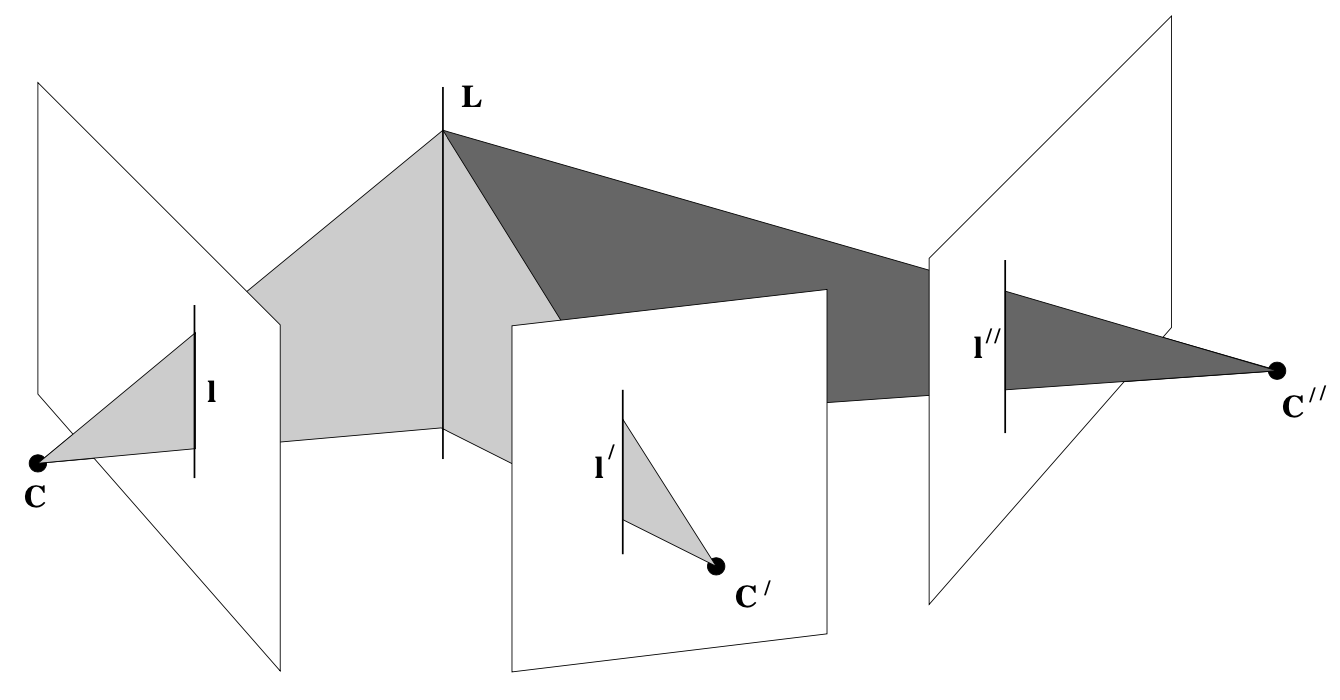
\includegraphics[width=0.5\textwidth]{Report/Figures/three-views.png}
	\caption[Trifocal Tensor Derivation]{A line L in 3-space is imaged as the corresponding triplet \( l \leftrightarrow l' \leftrightarrow l'' \) in three views indicated by their centres, \( C \), \( C' \) , \( C'' \) , and image planes. Conversely, corresponding lines back-projected from the first, second and third images all intersect in a single 3D line in space. \cite{1-multiple-view-geometry}}
\end{figure}

Considering projective transformations, we focus on properties such as image coordinates and 3D incidence relations, which remain invariant. Each image line is projected back to a plane, with these planes constrained to intersect at the common line in 3D space. This constraint is algebraically expressed by ensuring that a specific matrix \( M = [\pi, \pi', \pi''] \) has a rank of 2. Here, \( \pi \), \( \pi' \), and \( \pi'' \) represent the back-projected planes of the image lines in each view
\begin{equation}
	\pi = P^\top l = \left( \begin{array}{c} l \\ 0 \end{array} \right) \quad
	\pi' = P'^\top l' = \left( \begin{array}{c} A^\top l' \\ a_4^\top l' \end{array} \right) \quad
	\pi'' = P''^\top l'' = \left( \begin{array}{c} B^\top l'' \\ b_4^\top l'' \end{array} \right).
\end{equation}

The latter intersection constraint induces the following incidence relation amongst the image lines
\begin{equation}
	l_i = l'^\top \bm{T}_il'',
	\label{eq:incidenceRelation}
\end{equation}

where \( \bm{T}_i = a_ib_4^\top - a_4b_i^\top \), \( i = 1, 2, 3 \). The set of three matrices \( [\bm{T}_1, \bm{T}_2, \bm{T}_3] \) constitute the \ac{TFT} in matrix notation. Hence, the incidence relation (\ref{eq:incidenceRelation}) can be expressed as
\begin{equation}
	l^\top = l'^\top [\bm{T}_1, \bm{T}_2, \bm{T}_3] l''.
	\label{eq:incidenceRelationMatrix}
\end{equation}

\subsection{Tensor Notation}
Image points and lines are represented by homogeneous column and row 3-vectors, respectively. The \( ij \)-th entry of a matrix \( A \) is denoted by \( a_i^j \), index \( i \) being the contravariant (row) index and \( j \) being the covariant (column) index. If the canonical \( 3 \times 4 \) camera matrices are \( P = [I|0] \), \( P' = [a_j^i] \), and \( P'' = [b_j^i] \), the definition of the \acs{TFT} in tensor notation becomes
\begin{equation}
	\mathbfcal{T}_i^{jk} = a_i^jb_4^k - a_4^jb_i^k.
	\label{eq:tensorDef}
\end{equation}

The placement of indices in the tensor (two contravariant and one covariant) follows the arrangement of indices on the right side of the equation. Hence, the trifocal tensor is a mixed contravariant-covariant valency 3 tensor denoted by a homogeneous array of size \( 3 \times 3 \times 3 \) (\ie, 27 elements) and possesses 18 degrees of freedom.\\

Thus, the fundamental incidence relation (\ref{eq:incidenceRelation}) is expressed as
\begin{equation}
	l_i = l'_jl''_k\mathbfcal{T}_i^{jk}.
	\label{eq:incidenceRelationTensor}
\end{equation}

\subsection{Trilinearities}\label{sec:trilinearities}
Similarly to the fundamental matrix in two-view geometry, the trifocal tensor encodes relationships between points and lines across three perspectives. These relationships are denoted as trilinearities: "tri" since every monomial in the relation involves a coordinate from each of the three image elements involved, and linear because the relations are linear in each of the algebraic entities (\ie, the three arguments of the tensor). The following equation portrays a point-point-point (P-P-P) correspondence 
\begin{equation}
	[x']_{\times} \left( \sum_{i}x^i\bm{T}_i \right) [x'']_{\times} = 0_{3 \times 3},
	\label{eq:tftTrilinearities}
\end{equation}

with \( x \), \( x' \), and \( x'' \) being the homogeneous coordinates of corresponding points in three images. However, other trilinear relations can be derived, such as L-L-L, P-L-L, P-L-P, P-P-L, and P-P-P, where P stands for point and L stands for line. These trilinearities are invariant under projective transformations, ensuring robustness across different camera configurations and scenes.\\

Among the nine scalar equations in (\ref{eq:tftTrilinearities}), only four are linearly independent. They manifest linearity with respect to the parameters of the trifocal tensor and trilinearity with respect to the image coordinates. When viewed in pairs, the incidence relationships established by the fundamental matrices for the corresponding triplet \( x \), \( x' \), and \( x'' \) consist of a group of three equations that are linear with respect to the parameters of the fundamental matrices and bilinear with respect to the image points
\begin{equation}
	x_2^\top F_{21}x_1 = 0 \quad x_3^\top F_{31}x_1 = 0 \quad x_3^\top F_{32}x_2 = 0,
\end{equation}

where the involved fundamental matrices are
\begin{equation}
	F_{21} = [a_4]_{\times}A \quad F_{31} = [b_4]_{\times}B \quad F_{32} = [b_4 - BA^{-1}a_4]_{\times}BA^{-1}.
\end{equation}

\subsection{Linear Computation}
The trifocal tensor can be derived from a linear system described by the trilinear relationships outlined in (\ref{sec:trilinearities}). Each triplet yields nine equations that are linear with respect to the tensor's parameters, yet only four of these equations are linearly independent. To solve this linear system, a minimum of seven correspondences is required, with the additional constraint \( || \mathbfcal{T} || = 1 \). If more triplets are available, a solution minimizing the algebraic error can be obtained via Singular Value Decomposition (SVD). However, the resulting trifocal tensor may not always be valid.\\

To fix this, a valid trifocal tensor can be computed through an algebraic minimization algorithm that parallels the linear process employed to find the fundamental matrix.

\begin{algorithm}[h]
		\caption{Algebraic Minimization Algorithm (\acs{L-TFT})}
		\kwObjective{Given a set of point and line correspondences in three views, compute the trifocal tensor.}
		\kwAlgorithm{
		\begin{enumerate}[label=(\roman*),leftmargin=*,rightmargin=1.5em]
        	\item From the set of point and line correspondences compute the set of equations of the form \( At = 0 \), where \( t \) is the 27-vector made up of the entries of the trifocal tensor.
        	\item Solve these equations using the least-squares solution to constrained systems, in order to find an initial estimate of the trifocal tensor \( \mathbfcal{T}_i^{jk} \).
        	\item Find the two epipoles \( e' \) and \( e'' \) from \( \mathbfcal{T}_i^{jk} \) as the common perpendicular to the left null-vectors of the three slices \( \bm{T}_i \).
        	\item Construct the \( 27 \times 18 \) matrix \( E \) such that \( t = Ea \), where a is the vector representing entries of \( a_i^j \) and \( b_i^k \), and where \( E \) espresses the linear relationship \( \mathbfcal{T}_i^{jk} = a_i^j{e''}^k - {e'}^jb_i^k \).
        	\item Minimize \( || AEa || \) subject to \( || Ea || = 1 \). Compute the error vector \( \epsilon = AEa \).
        	\item \textbf{Iteration:} The mapping \( (e', e'') \mapsto \epsilon \) is a mapping from \( \mathbb{R}^6 \) to \( \mathbb{R}^{27} \). Iterate on the last two steps with varying \( e' \) and \( e'' \) using the \ac{LM} algorithm to find the optimal \( e' \), \( e'' \) pair. Hence find the optimal \( t = Ea \) containing the entries \( \mathbfcal{T}_i^{jk} \).
    	\end{enumerate}
    }
    \label{algo:LTFT}
\end{algorithm}

\subsection{Optimization}
Several concise and consistent descriptions of the trifocal tensor have been suggested in prior literature \cite{4-minimal-constraints-tft, 5-nonlinear-three-view-estimation, 3-tft-vs-fund, 6-nordberg-param, 7-faugeras-papadopoulo-param, 8-ponce-hebert-param, 9-ressl-param, 10-robust-param}, where the term consistent ensures that the tensor does satisfy its constraints, thus is geometrically valid. We've opted to concentrate on four representative ones that can be seamlessly integrated into the pose estimation procedure, exploiting \acs{GH}.

\begin{algorithm}[h]
		\caption{\acs{GH} Algorithm for the \acs{TFT} (\acs{R-TFT}, \acs{N-TFT}, \acs{FP-TFT}, \acs{PH-TFT})}
		\kwObjective{Given a set of point and line correspondences in three views, compute the trifocal tensor.}
		\kwAlgorithm{
		\begin{enumerate}[label=(\roman*),leftmargin=*,rightmargin=1.5em]
        	\item \textbf{Initial Linear Estimation:} Algorithm (\ref{algo:LTFT}).
        	\item \textbf{Optimization:} Apply \acs{GH} with respect to one of the parametrizations to iteratively reduce the estimation error.
        \end{enumerate}
    }
\end{algorithm}

\paragraph{Ressl (\acs{R-TFT})}
Ressl, in his thesis \cite{9-ressl-param}, introduced a minimal parameterization for the trifocal tensor, relying on algebraic constraints within correlation slices. This formulation consists of 20 parameters and 2 constraints. It enables the comprehensive characterization of the trifocal tensor for three views. The trifocal tensor, represented by the three matrices \( T_i \), can be succinctly parameterized as follows
\begin{equation}
	\bm{T}_i = [s_i, vs_i + m_ie_{31}, ws_i + n_ie_{31}]^\top,
\end{equation}

where \( s_i \in \mathbb{R}^3 \) are such that \( || (s_1 s_2 s_3) || = 1 \), \( e_{31} \in \mathbb{R} \) with \( || e_{31} || = 1 \), and \( v, w, m_i, n_i \in \mathbb{R} \).\\

This parameterization directly links to the epipoles: where \( e_{31} = b_4 \) signifies the epipole, the projection of the first camera center onto the third image, and \( e_{21} = a_4 \) is proportionate to \( (1,v,w)^\top \). Moreover, it's tied to an equivalent parameterization of three canonical projective matrices.

\paragraph{Nordberg (\acs{N-TFT})}
Another approach to parameterize the trifocal tensor involves three \( 3 \times 3 \) orthogonal matrices, \( U \), \( V \), and \( W \), as mentioned in \cite{6-nordberg-param}. These matrices transform the original tensor into a sparse form, denoted as \( \bm{\widetilde{\mathbfcal{T}}} \), containing only 10 non-zero parameters, up to scale
\begin{equation}
	\bm{\widetilde{\mathbfcal{T}}} = \mathbfcal{T} (U \otimes V \otimes W),
\end{equation}

where the tensor operation \( \otimes \) corresponds to the matrix operation on the slices \( \widetilde{T_i} = V^\top (\sum_{m}U_{m,i}T_m) W \). The scale can be fixed by imposing \( || \bm{\widetilde{\mathbfcal{T}}} || = 1 \).\\

For canonical cameras, such orthogonal matrices can be computed as
\begin{equation}
	\begin{gathered}
		U_0 = (A^{-1}a_4, {[A^{-1}a_4]_{\times}}^2B^{-1}b_4, [A^{-1}a_4]_{\times}B^{-1}b_4)\\
		U = U_0(U_0^\top U_0)^{-\frac{1}{2}}\\
		V_0 = (a_4, [a_4]_{\times}AB^{-1}b_4, {[a_4]_{\times}}^2AB^{-1}b_4)\\
		V = V_0(V_0^\top V_0)^{-\frac{1}{2}}\\
		W_0 = (b_4, [b_4]_{\times}BA{-1}a_4, {[b_4]_{\times}}^2BA^{-1}a_4)\\
		W = W_0(W_0^\top W_0)^{-\frac{1}{2}},
	\end{gathered}
\end{equation}

and each matrix can be represented by 3 parameters, resulting in a total of 19 parameters for the trifocal tensor \( \mathbfcal{T} \), along with one constraint to determine the scale of \( \bm{\widetilde{\mathbfcal{T}}} \).\\

However, a notable drawback of this particular parameterization arises when the camera centers are collinear. In such cases, the matrices \( U_0 \), \( V_0 \), and \( W_0 \) become singular, rendering it impossible to compute orthogonal matrices from them. Consequently, this parameterization is only applicable when the camera centers are non-collinear.

\paragraph{Faugeras and Papadopoulo (\acs{FP-TFT})}
The work outlined in \cite{7-faugeras-papadopoulo-param} introduces a set of 12 algebraic equations, serving as constraints to fully define a trifocal tensor. These include three constraints of third-degree, corresponding to the slices' determinants being zero, \( |T_i| = 0 \) for \( i \in \{1, 2, 3\} \), and an additional nine constraints of sixth-degree. These sixth-degree constraints involve combinations of various determinants of the tensor's elements
\begin{equation}
	\begin{gathered}
		| \bm{T}_.^{j_1}{k_1}\bm{T}_.^{j_1}{k_2}\bm{T}_.^{j_2}{k_2} | | \bm{T}_.^{j_1}{k_1}\bm{T}_.^{j_2}{k_1}\bm{T}_.^{j_2}{k_2} | -\\
		| \bm{T}_.^{j_2}{k_1}\bm{T}_.^{j_1}{k_2}\bm{T}_.^{j_2}{k_2} | | \bm{T}_.^{j_1}{k_1}\bm{T}_.^{j_2}{k_2}\bm{T}_.^{j_1}{k_2} | = 0,
	\end{gathered}
\end{equation}

where \( j_1, j_2, k_1, k_2 \in \{1, 2, 3\} \) with \( j_1 \neq j_2 \) and \( k_1 \neq k_2 \), and where \( \bm{T}_.^{jk} \) represents the vector \( (\bm{T}_1^{jk}, \bm{T}_2^{jk}, \bm{T}_3^{jk})^\top \).\\

This collection isn't minimal because it requires just 9 constraints to fully define a valid trifocal tensor. The authors suggest a method for achieving a minimal parameterization using these constraints, which involves solving a second-degree polynomial, resulting in two potential tensors. We find it preferable to pursue constraint minimization rather than minimal parameters for a simpler implementation.

\paragraph{Ponce and Hebert \( \bm{\Pi} \) Matrices (\acs{PH-TFT})}
An alternative method of characterizing the 3-view model has been investigated in \cite{8-ponce-hebert-param}. By analyzing how three lines intersect in space, a trio of matrices has been derived, each associated with principal lines. These matrices, comprising a total of 27 parameters, impose constraints on the correspondence between three image points. Analogous to the TFT, they serve a crucial role. For a configuration involving three cameras with non-collinear centers and three image points, denoted as \( x_1 \), \( x_2 \), and \( x_3 \), there exist three \( 4 \times 3 \) matrices, denoted as \( \Pi_i = (\pi_{1i}, \pi_{2i}, \pi_{3i}, \pi_{4i})^\top \), each scalable, where \( \pi_{ii} = (0 0 0)^\top \), and they satisfy

\begin{equation}
	x_1^\top (\pi_{41}\pi_{32}\top - \pi_{31}\pi_{42}\top) x_2 = 0
	\label{eq:phConst1}
\end{equation}
\begin{equation}
	x_1^\top (\pi_{41}\pi_{23}\top - \pi_{21}\pi_{43}\top) x_3 = 0
	\label{eq:phConst2}
\end{equation}
\begin{equation}
	x_3^\top (\pi_{43}\pi_{13}\top - \pi_{12}\pi_{43}\top) x_3 = 0
	\label{eq:phConst3}
\end{equation}
\begin{equation}
	(\pi_{21}^\top x_1) (\pi_{32}^\top x_2) (\pi_{13}^\top x_3) = (\pi_{31}^\top x_1) (\pi_{12}^\top x_2) (\pi_{23}^\top x_3),
	\label{eq:phConst4}
\end{equation}

if, and only if, the \( x_i \) form a triplet of corresponding points.\\
Ponce and Hebert propose the 6 following homogeneous constraints
\begin{equation}
	\begin{gathered}
		\pi_{21}^1 = \pi_{32}^2 = \pi_{13}^3 = ,0\\
		\pi_{31}^2 = \pi_{41}^3, \quad \pi_{12}^3 = \pi_{42}^1, \quad \pi_{23}^1 = \pi_{43}^2.
	\end{gathered}
\end{equation}

This can be accomplished through a projective transformation of the space, reducing the parameters to 21. By imposing three norm constraints on the matrices, \( || \Pi_i || = 1 \), we achieve the most concise representation.\\

Analogous to the trilinearities (\ref{eq:tftTrilinearities}) in the trifocal tensor scenario, these parameters yield four equations detailing the incidence relation for image points. Equations (\ref{eq:phConst1}), (\ref{eq:phConst2}), and (\ref{eq:phConst3}) are bilinear regarding the points and are entirely analogous to the epipolar equations provided by the fundamental matrices. Equation (\ref{eq:phConst4}), however, is trilinear concerning the image points, playing a pivotal role in characterizing the correspondence of three points that fundamental matrices falter at when one point resides on the line connecting two epipoles. This underscores the geometric significance of leveraging three views instead of individual pairs in characterizing matches.\\

Much like Nordberg's parameterization of the trifocal tensor, a primary limitation of the \( \Pi \) matrices is their applicability solely to non-collinear camera centers. In instances of collinear camera centers, Ponce and Hebert also proposed equivalent matrices incorporating an additional trilinear constraint.

\section{Pose Estimation}\label{sec:estimation}
We can derive the epipoles, which are the projections of the first camera centre onto the second and third images, from a \acs{TFT} \( \mathbfcal{T} \). The epipole \( e_{21} \) is found as the common point of intersection among the lines represented by the left null-vectors of \( \bm{T}_1 \), \( \bm{T}_2 \), and \( \bm{T}_3 \). Similarly, the epipole \( e_{31} \) is determined as the shared point of intersection among the lines represented by the right null-vectors of \( \bm{T}_1 \), \( \bm{T}_2 \), and \( \bm{T}_3 \). Subsequently, we can compute the \acs{FM}s as
\begin{equation}
	\begin{gathered}
		F_{21} = [e_{21}]_{\times}[\bm{T}_1e_{31}, \bm{T}_2e_{31}, \bm{T}_3e_{31}]\\
		F_{31} = [e_{31}]_{\times}[\bm{T}_1^\top e_{21}, \bm{T}_2^\top e_{21}, \bm{T}_3^\top e_{21}].
	\end{gathered}
	\label{eq:fmFromEpiTFT}
\end{equation}

The \ac{EM} is the specialisation of the \acs{FM} to the case of normalized image coordinates. The \acs{EM}s here can be derived from \( F_{21}, F_{31} \), and the calibration matrices \( K_i \), using the formula \( [t_{ij}]_{\times}R_{ij} = E_{ij} = K_i^\top F_{ij}K_j \). From these \acs{EM}s, the relative orientations \( (R_{21}, t_{21}) \) and \( (R_{31}, t_{31}) \) can be extracted through the \acs{SVD} of \( E_{21} \) and \( E_{31} \), with each translation vector's scale remaining unknown. To establish an overall scale, we set \( \Vert t_{21} \Vert = 1 \), while the relative scale \( \lambda \) of \( t_{31} \) can be determined by triangulating the space points \( \{X^n\}_n \) from the first two cameras' projections and minimizing the algebraic error relative to the third image, as shown
\begin{equation}
	\argmin_{\lambda \in \mathbb{R}}{\sum_{n = 1}^{N}{\left\Vert x_3^n \times \left( K_3 \left( R_{31}X^n + \lambda \frac{t_{31}}{\Vert t_{31} \Vert} \right) \right) \right\Vert}}.
\end{equation}

The latter admits a closed form solution. So, either from the \acs{TFT} or the \acs{FM}s, we possess a method for computing the camera poses.

\subsection{Bundle Adjustment}
In pose estimation, a frequent final stage involves refining the orientations through \ac{BA}. This process aims to minimize the square reprojection error across potential camera orientations and spatial points. For N correspondences and M = 3 cameras
\begin{equation}
	\min_{\{ R_j, t_j \}_j, \{ X^i \}_i}{\epsilon^2}, \quad \epsilon^2 = \sum_{i = 1}^{N}{\sum_{j = 1}^{M}{d \left( x_j^i, K_j(R_jX^i + t_j) \right)^2}},
	\label{eq:baMin}
\end{equation}

where \( x_j^i \) is for the homogeneous coordinates of the observed image point, and the distance \( d \) is the Euclidean distance in homogeneous coordinates
\begin{equation}
	d \left( (x, y, z)^\top, (t, u, v)^\top \right)^2 = \left( \frac{x}{z} - \frac{t}{v} \right)^2 + \left( \frac{y}{z} - \frac{u}{v} \right)^2.
\end{equation}

The optimization procedure can be executed using the \acs{LM} algorithm \cite{14-levenberg}.

\begin{algorithm}[h]
		\caption{Pose Estimation Algorithm}
		\kwObjective{Given \acs{FM} or \acs{TFT}, extract camera poses.}
		\kwAlgorithm{
		\begin{enumerate}[label=(\roman*),leftmargin=*,rightmargin=1.5em]
        	\item If employing \acs{TFT}, derive the epipoles \( e_{21}, e_{31} \) first, and then compute the fundamental matrices \( F_{21}, F_{31} \) as stated in Equation (\ref{eq:fmFromEpiTFT}); otherwise (employing \acs{FM}) go to step (ii).
        	\item Compute essential matrices \( E_{21}, E_{31} \) from the fundamental matrices \( F_{21}, F_{31} \) and the calibration matrices \( K_i \).
        	\item Exploit essential matrices to determine rotations \( R_2, R_3 \) and translations \( t_2, t_3 \).
        	\item Apply \acs{BA} to refine rotations and translations (\ie, orientations), by minimizing the squared reprojection error as stated in Equation (\ref{eq:baMin}).
        	\item Triangulate 3D points from their image projections using the \ac{DLT} algorithm, obtaining the reconstructed 3D scene.
        \end{enumerate}
    }
\end{algorithm}

\pagebreak

\section{Experiments}\label{sec:experiments}
We put into action and assessed the outcomes of pose estimation for both synthetic and real data employing both the fundamental matrix and the trifocal tensor. \footnote{The MATLAB code to reproduce these experiments is available at the GitHub repository: \href{https://github.com/versi379/Two-View-Three-View-Pose-Estimation.git}{https://github.com/versi379/Two-View-Three-View-Pose-Estimation.git}.}

As for the \acs{FM}, we compute it both linearly (\acs{L-FM}) and through \acs{GH} (\acs{O-FM}), whereas for the \acs{TFT} we employ linear computation (\acs{L-TFT}) and apply \acs{GH} using minimal parametrizations proposed by Ressl (\acs{R-TFT}), Nordberg (\acs{N-TFT}), Faugeras \& Papadopoulo (\acs{FP-TFT}), and Ponce \& Hebert (\acs{PH-TFT}).

Additionally, we present the result obtained through \acs{BA}, which is initialised using any of the aforementioned methods. Remarkably, our experiments reveal that all initialisations yield nearly identical final poses post-minimization in the majority of cases, an observation we delve into later in our discussions.

\subsection{Synthetic Data}
We conducted trials on synthetic data to assess pose estimation using both the fundamental matrix and the trifocal tensor across various configurations. The standard experimental setup consists of a collection of spatial points situated within a 400mm-sided cube centred at the world's origin, as shown in Figure (\ref{fig:syntheticScenes}). Points are projected onto three views, and Gaussian noise with a standard deviation of 1 pixel is applied to the image points, unless specified otherwise. A set of 10 points is utilised for computations across various models. The image dimensions are \( 1800 \times 1200 \) pixels, representing a sensor size of \( 36mm \times 24mm \), with a fixed focal length of 50mm. All cameras are aligned to focus on the origin. Results are averaged over 30 simulations of data.\\

\begin{figure}[h]
    \centering
    \subfigure[]{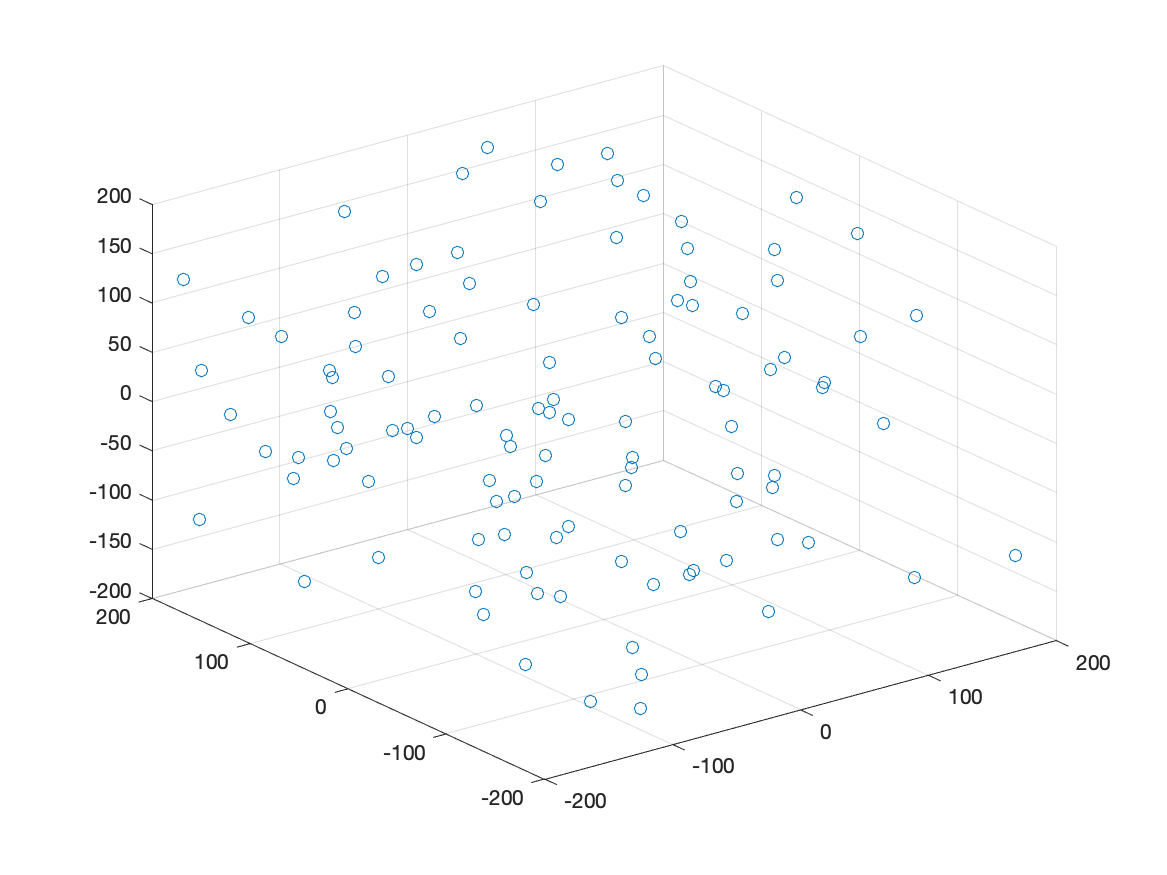
\includegraphics[width=0.34\textwidth]{Experiments/Synthetic/scene/IT1.png}} 
    \subfigure[]{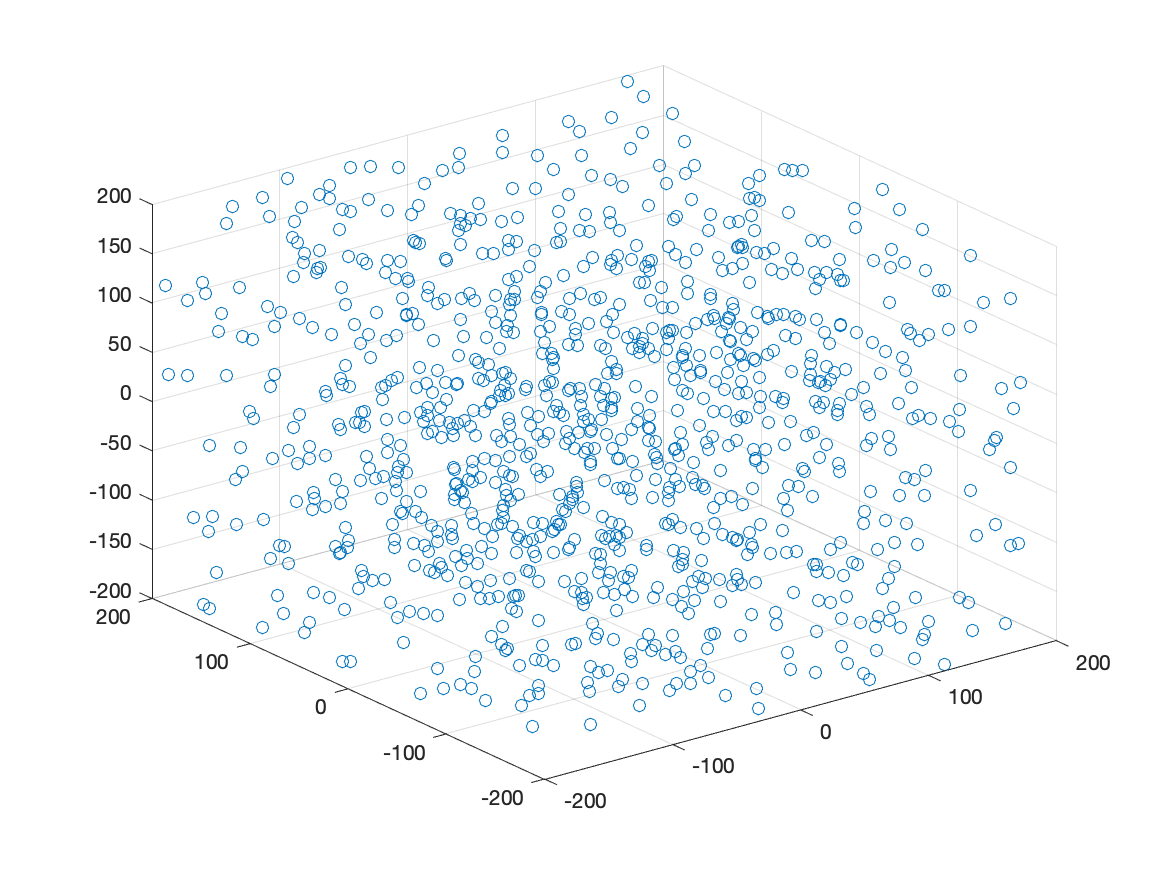
\includegraphics[width=0.34\textwidth]{Experiments/Synthetic/scene/IT10.png}}
    \\ 
    \subfigure[]{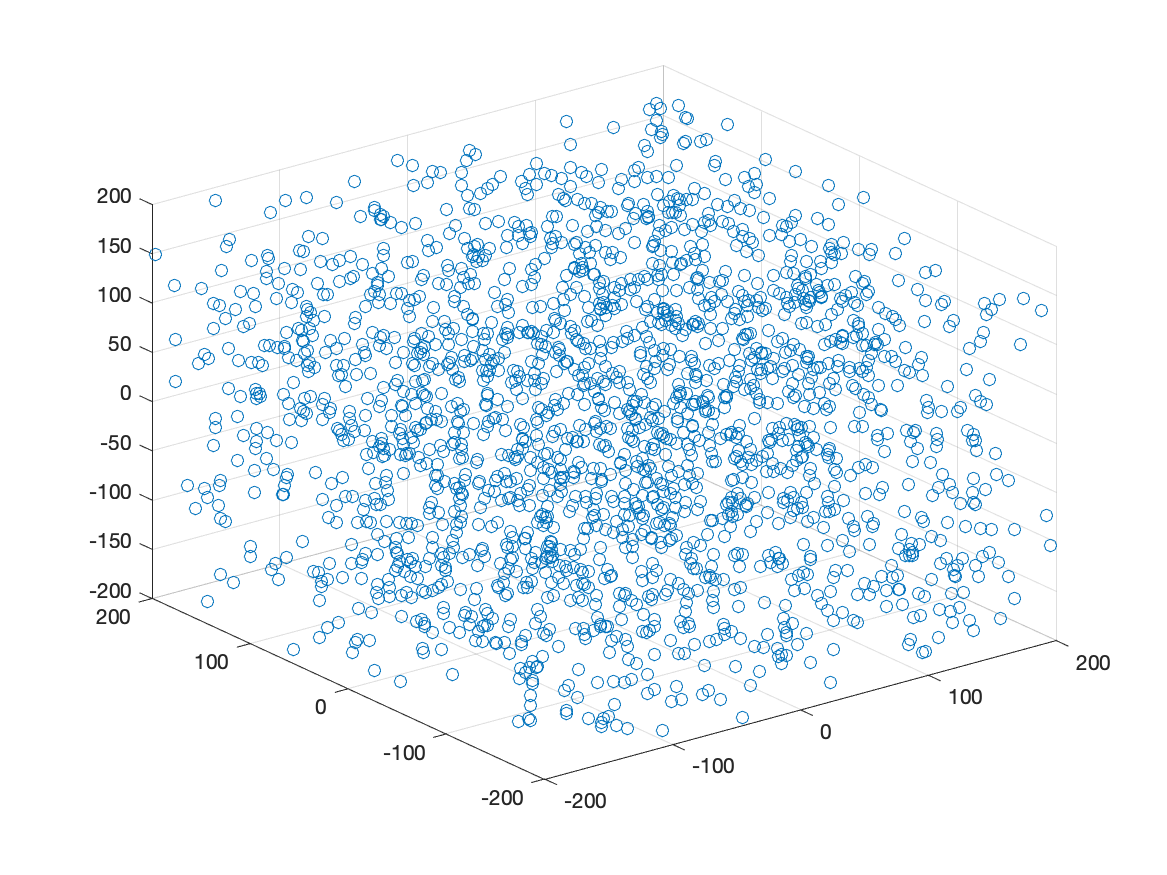
\includegraphics[width=0.34\textwidth]{Experiments/Synthetic/scene/IT20.png}}
    \subfigure[]{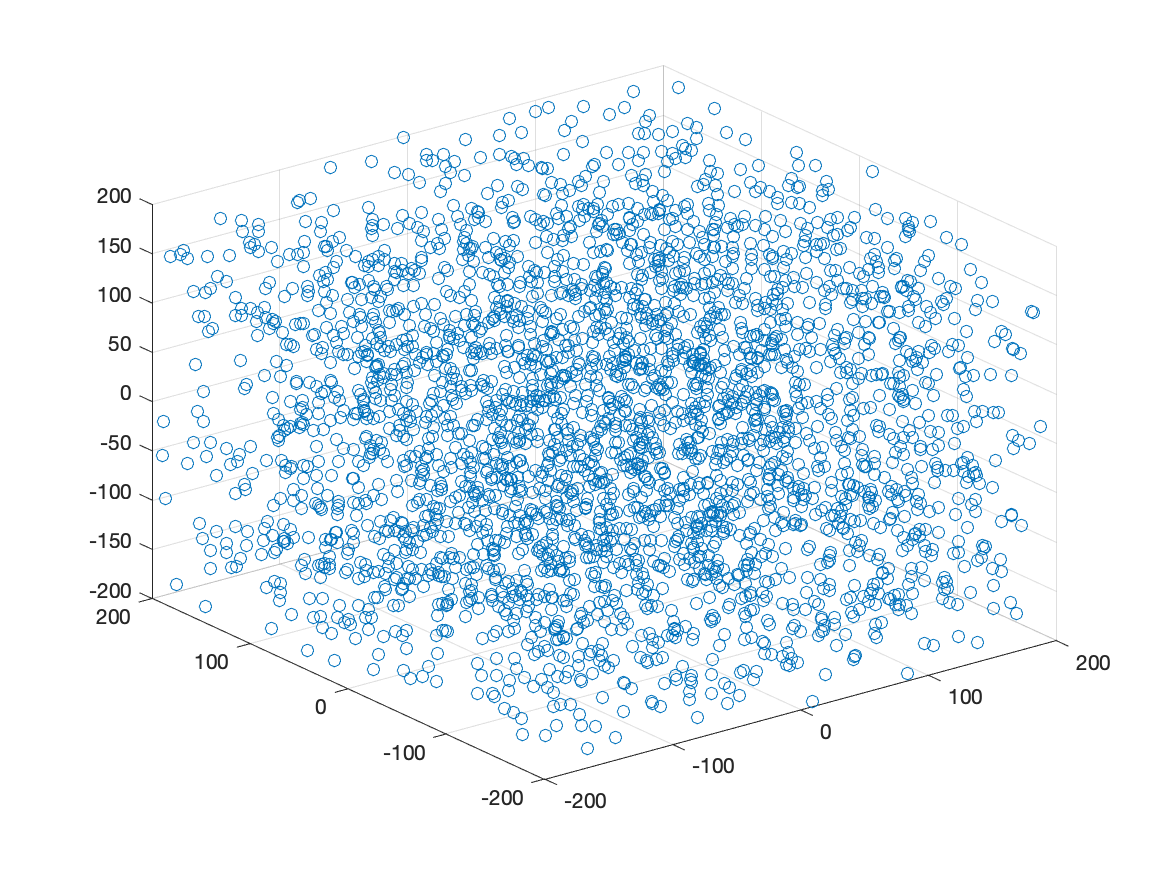
\includegraphics[width=0.34\textwidth]{Experiments/Synthetic/scene/IT30.png}}
    \caption[Synthetic Scene Setup]{Set of 3D points considered in the synthetic experiment setup: (a) 100 points simulation, (b) 1000 points simulation, (c) 2000 points simulation, (d) 3000 points simulation.}
    \label{fig:syntheticScenes}
\end{figure}

% to put image of synthetic points
\pagebreak

% Varying noise discussion
\subsubsection*{Metrics varying Noise}
Metrics before and after Bundle Adjustment, against Gaussian noise level added to the data points, are shown respectively in Figure (\ref{fig:initNoisePlot}) and Figure (\ref{fig:BANoisePlot}).

Initially, all methods show increasing reprojection, rotation, and translation errors as noise rises, with \acs{FP-TFT} and \acs{O-FM} demonstrating the lowest errors, indicating higher accuracy. Conversely, \acs{L-TFT} and \acs{R-TFT} exhibit higher errors, suggesting less robustness to noise. The number of iterations generally increases with noise, with \acs{N-TFT} requiring the most iterations, and \acs{L-TFT} showing the fastest computation times.

However, after \acs{BA}, all methods display significantly reduced errors and a linear increase with noise, indicating improved precision and robustness. The number of iterations and computational times remain relatively stable post-adjustment, demonstrating efficient optimisation. Overall, these plots highlight a trade-off between accuracy and computational efficiency, with bundle adjustment enhancing performance across all methods, making them more precise and robust to noise.\\

% Varying focal length discussion
\subsubsection*{Metrics varying Focal Length}
Metrics before and after Bundle Adjustment, against Gaussian noise level added to the data points, are shown respectively in Figure (\ref{fig:initNoisePlot}) and Figure (\ref{fig:BANoisePlot}).

Before \acs{BA}, the \acs{TFT} methods generally showed higher errors than the \acs{FM} methods. The \acs{L-TFT} had the highest initial errors in reprojection, rotation, and translation, while both the \acs{L-FM} and \acs{O-FM} performed better in initial estimates.

After applying \acs{BA}, the differences between parametrizations became less pronounced, especially for reprojection and rotation errors. The \acs{FP-TFT} and \acs{PH-TFT} methods seemed to perform consistently well across different metrics. The \acs{L-TFT}, while greatly improved, still showed higher errors and computation time in some cases compared to other parametrizations.\\

% Varying number of points discussion
\subsubsection*{Metrics varying Number of Points}
Metrics before and after Bundle Adjustment, against the number of points considered in the synthetic scene, are shown respectively in Figure (\ref{fig:initPointsPlot}) and Figure (\ref{fig:BAPointsPlot}).

Pre-\acs{BA} performances showed errors (reprojection, rotation, translation) being significantly higher for all methods, especially with a small number of points. The \acs{L-TFT} method generally showed the highest initial errors, whereas both the \acs{FM} methods often performed better in initial estimates.

Post-\acs{BA} performances showed error significantly reduced, with reprojection error decreasing from hundreds to less than 0.1 pixels, and rotation \& translation errors reduced to near-zero.

% Varying angle discussion
\subsubsection*{Metrics varying Camera Angle}
Metrics before and after Bundle Adjustment, against the varying angle among the three camera centers, are shown respectively in Figure (\ref{fig:initAnglePlot}) and Figure (\ref{fig:BAAnglePlot}).

Again, results after \acs{BA} are clearly more accurate with respect to the initial ones, with errors being almost null for all methods except \acs{N-TFT}, which shows peaks for certain angular values.

\begin{figure}[p]
	\centering
	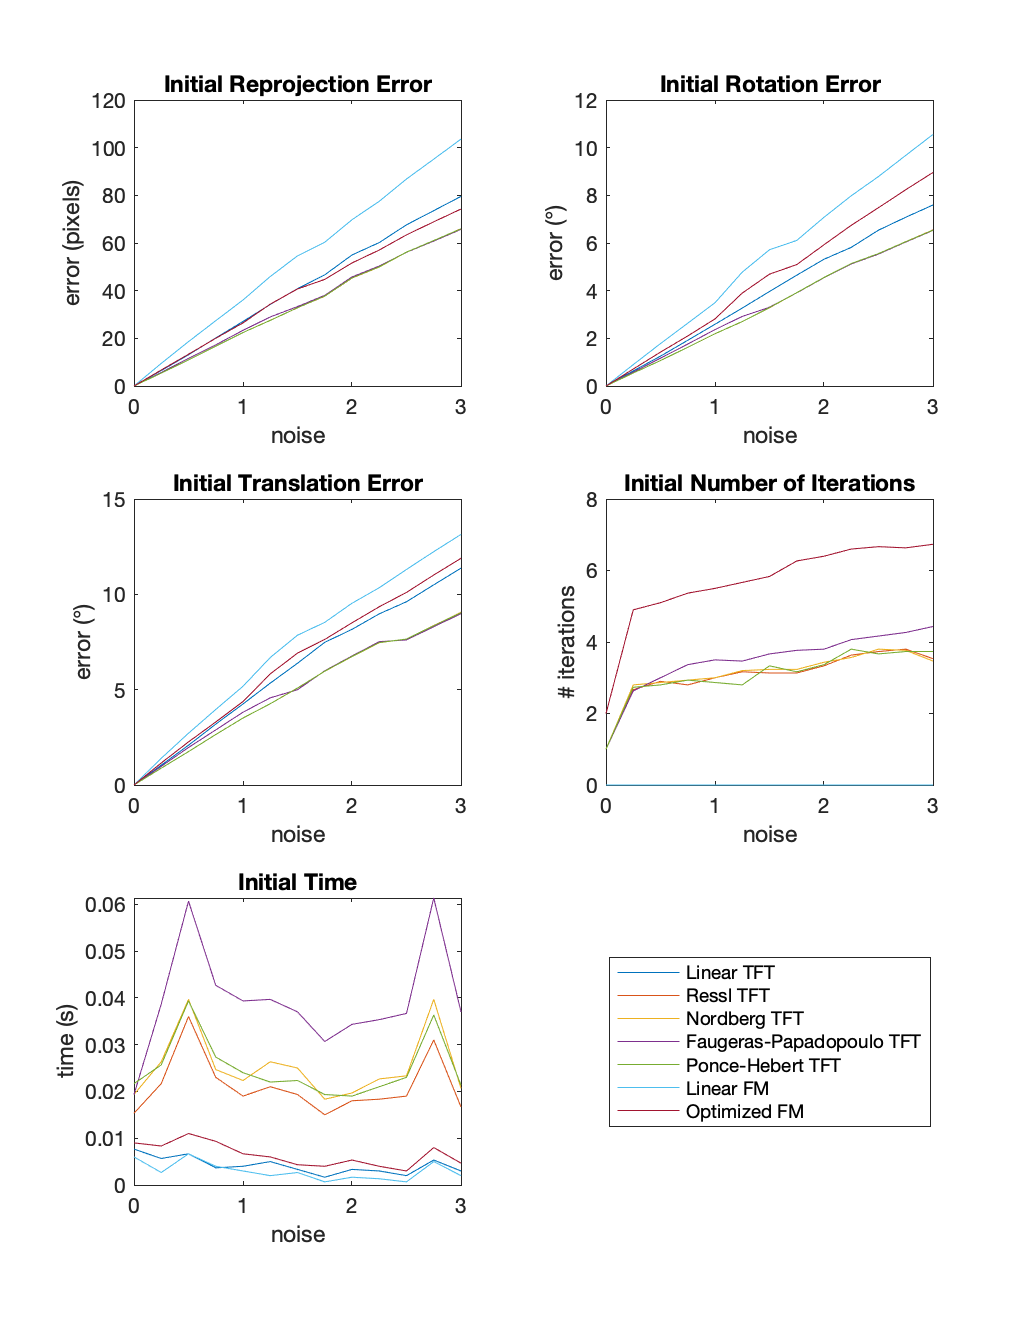
\includegraphics[width=1\textwidth]{Experiments/Synthetic/noise/INITnoisePlots.png}
	\caption[Synthetic Trial varying Gaussian Noise]{Initial reprojection error (top-left), rotation error (top-right), translation error (mid-left), number of iterations (mid-right), computational time (bottom-left); when varying the Gaussian noise added to the image points.}
	\label{fig:initNoisePlot}
\end{figure}

\begin{figure}[p]
	\centering
	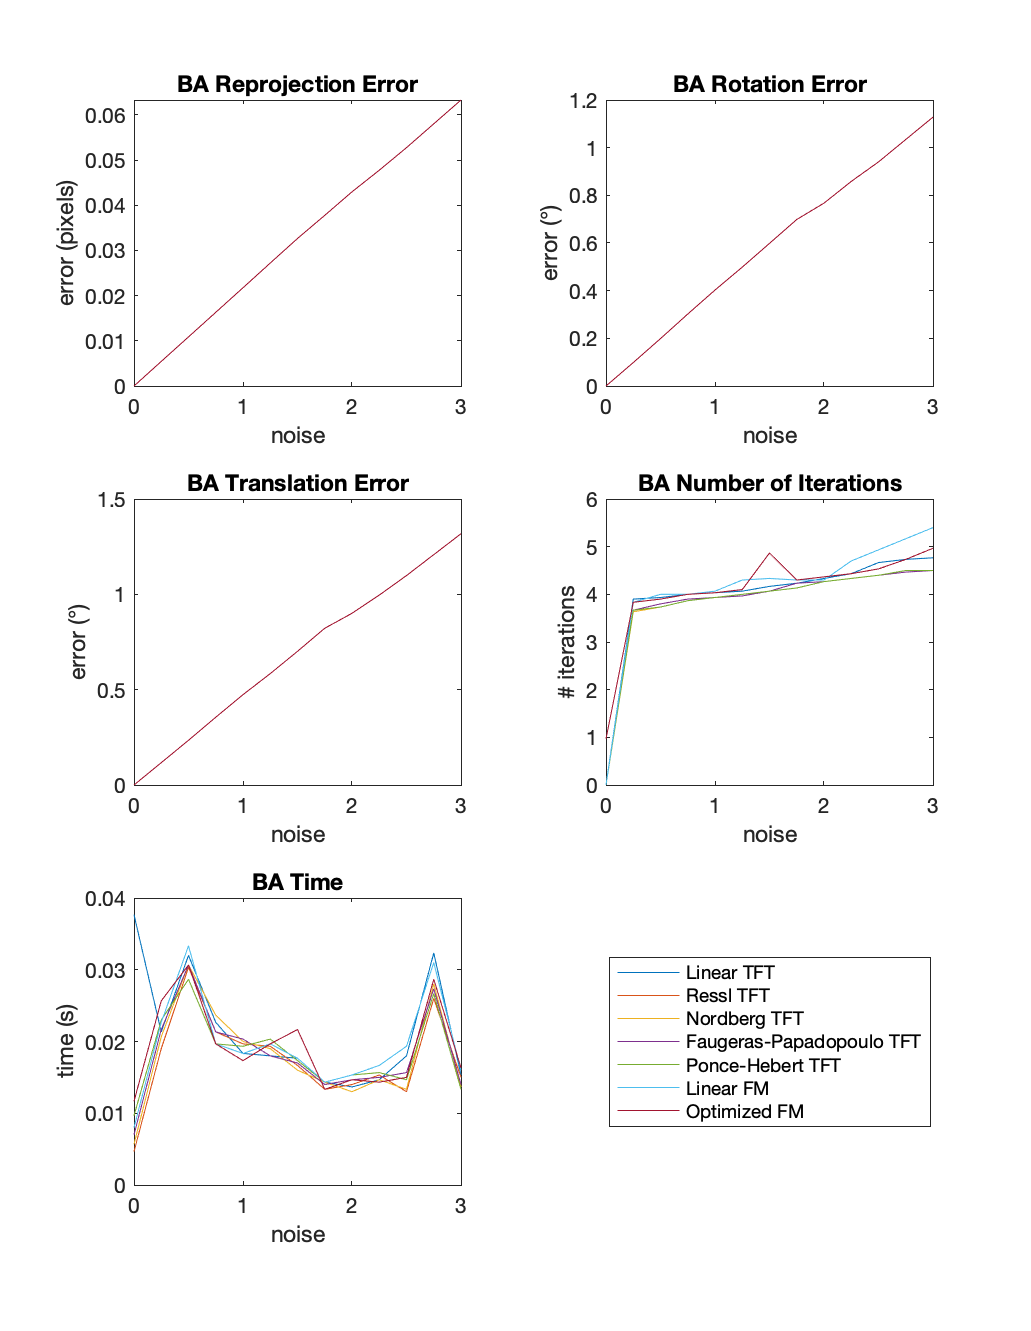
\includegraphics[width=1\textwidth]{Experiments/Synthetic/noise/BAnoisePlots.png}
	\caption[Synthetic Trial varying Gaussian Noise with \acs{BA}]{Reprojection error (top-left), rotation error (top-right), translation error (mid-left), number of iterations (mid-right), computational time (bottom-left) after \acs{BA}; when varying the Gaussian noise added to the image points.}
	\label{fig:BANoisePlot}
\end{figure}

\begin{figure}[p]
	\centering
	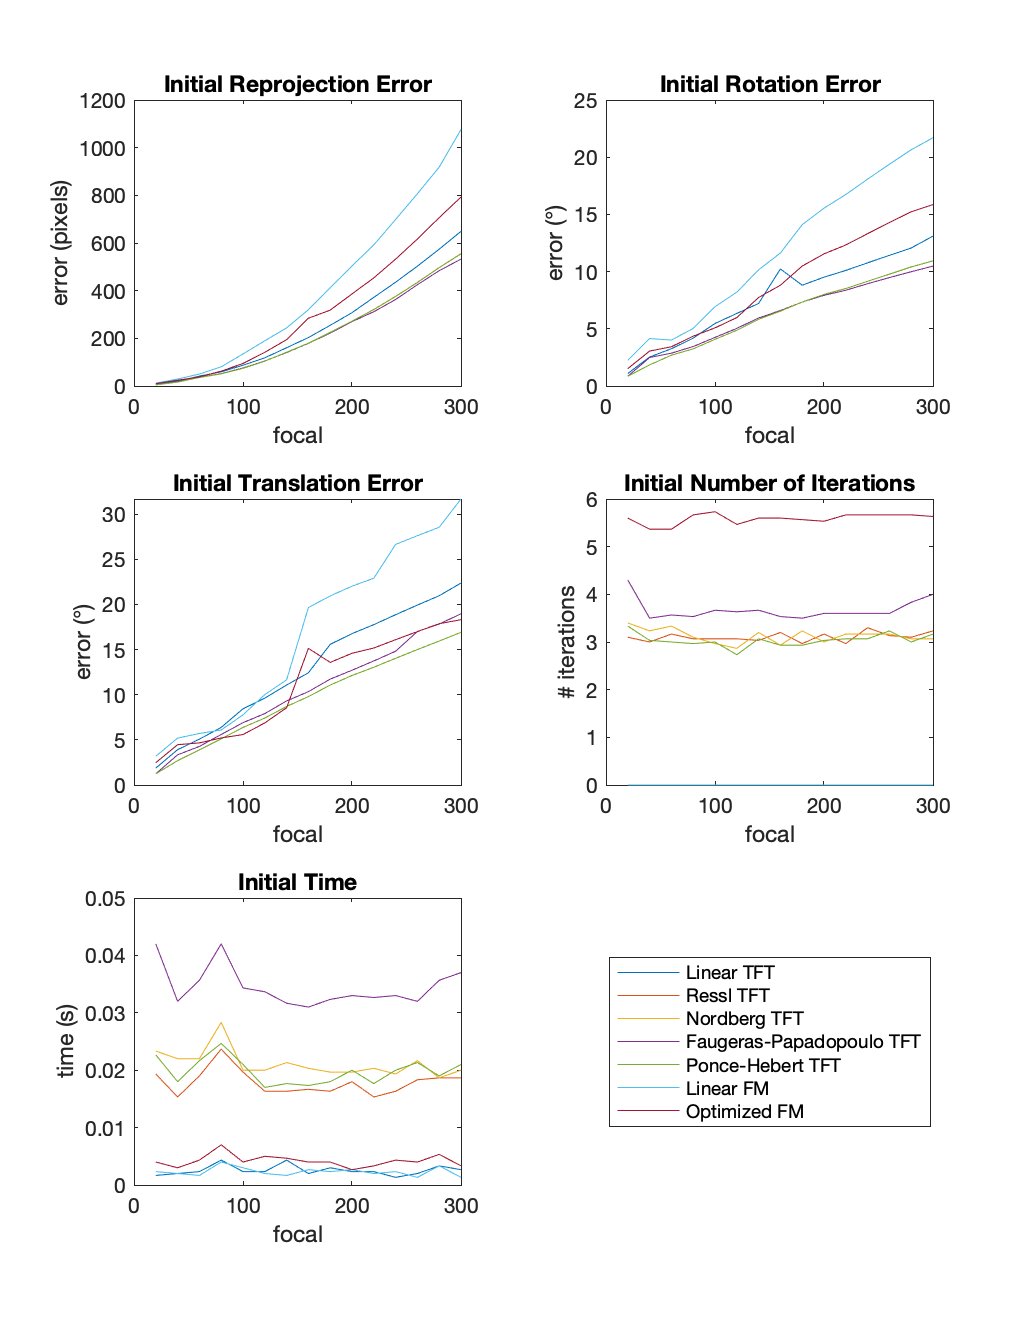
\includegraphics[width=1\textwidth]{Experiments/Synthetic/focal/INITfocalPlots.png}
	\caption[Synthetic Trial varying Focal Length]{Initial reprojection error (top-left), rotation error (top-right), translation error (mid-left), number of iterations (mid-right), computational time (bottom-left); when varying the focal length.}
	\label{fig:initFocalPlot}
\end{figure}

\begin{figure}[p]
	\centering
	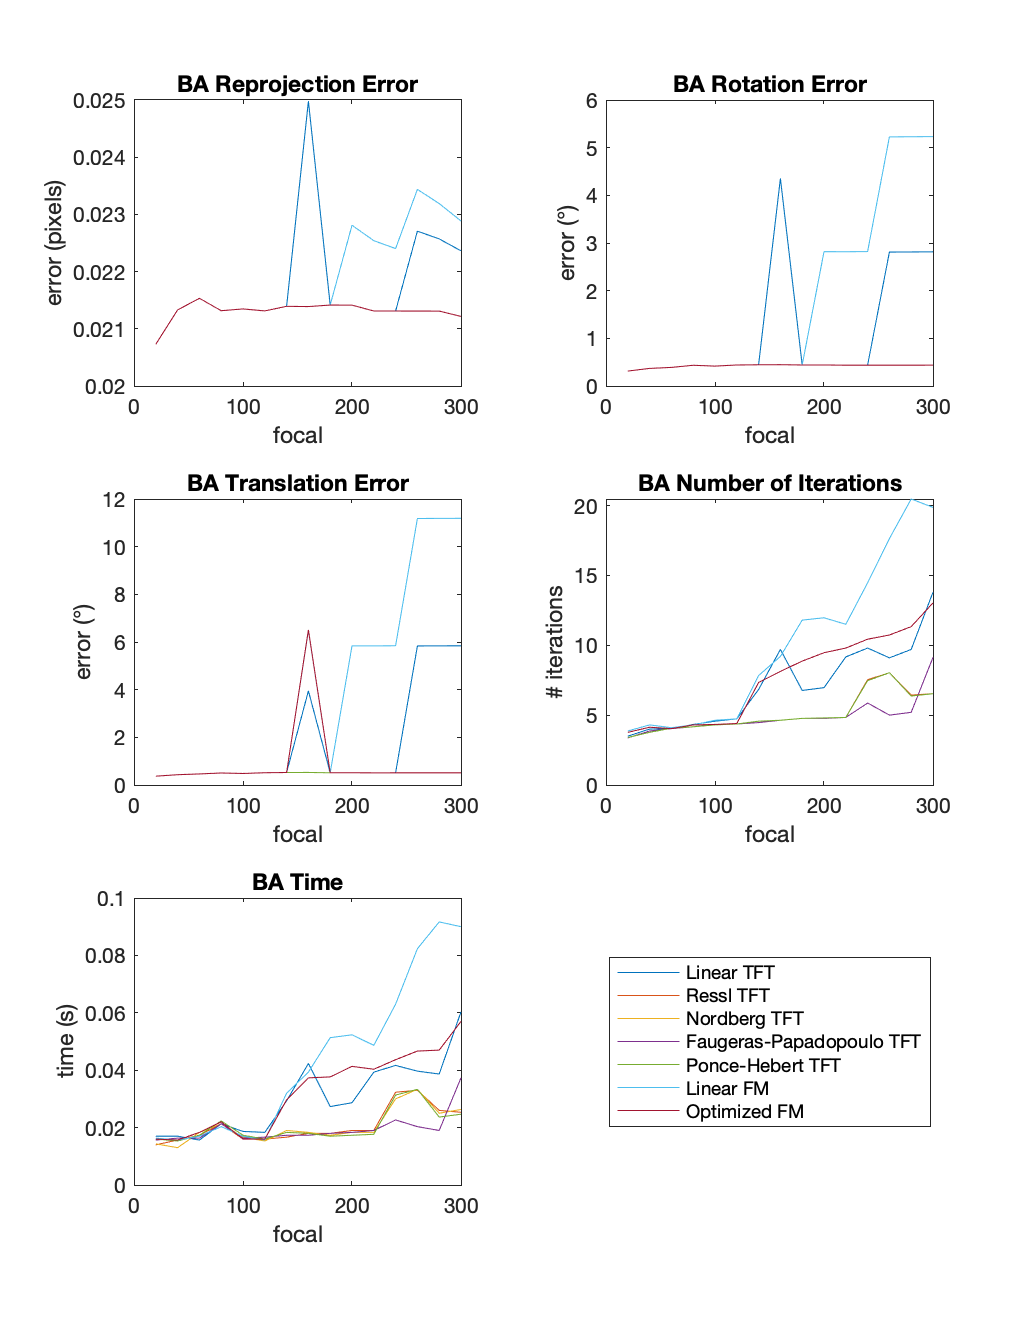
\includegraphics[width=1\textwidth]{Experiments/Synthetic/focal/BAfocalPlots.png}
	\caption[Synthetic Trial varying Focal Length with \acs{BA}]{Reprojection error (top-left), rotation error (top-right), translation error (mid-left), number of iterations (mid-right), computational time (bottom-left) after \acs{BA}; when varying the focal length.}
	\label{fig:BAFocalPlot}
\end{figure}

\begin{figure}[p]
	\centering
	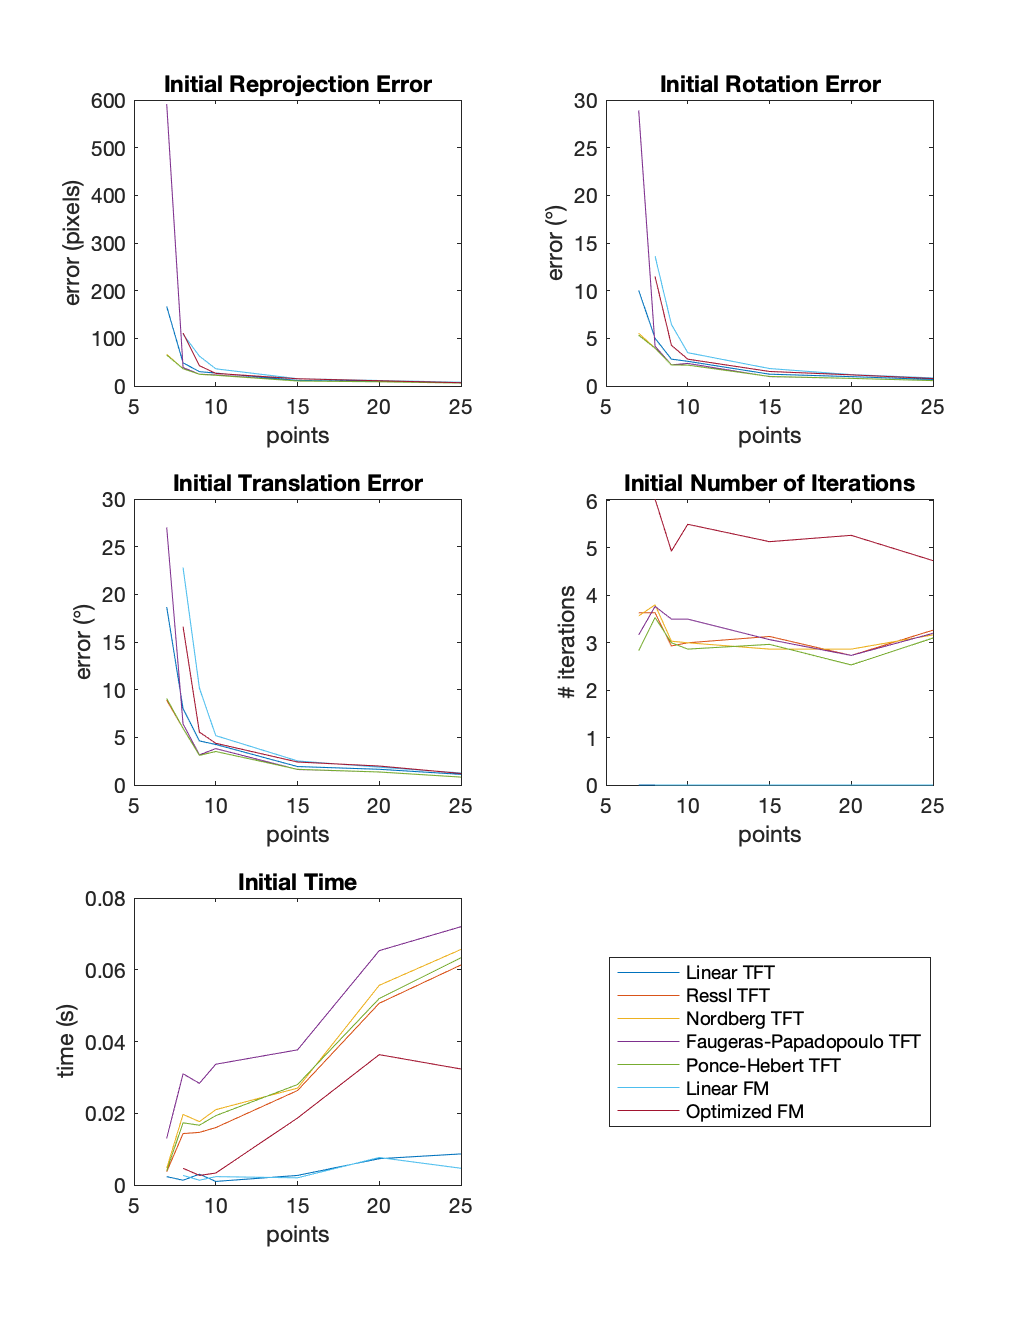
\includegraphics[width=1\textwidth]{Experiments/Synthetic/points/INITpointsPlots.png}
	\caption[Synthetic Trial varying Number of Image Points]{Initial reprojection error (top-left), rotation error (top-right), translation error (mid-left), number of iterations (mid-right), computational time (bottom-left); when varying the number of image points.}
	\label{fig:initPointsPlot}
\end{figure}

\begin{figure}[p]
	\centering
	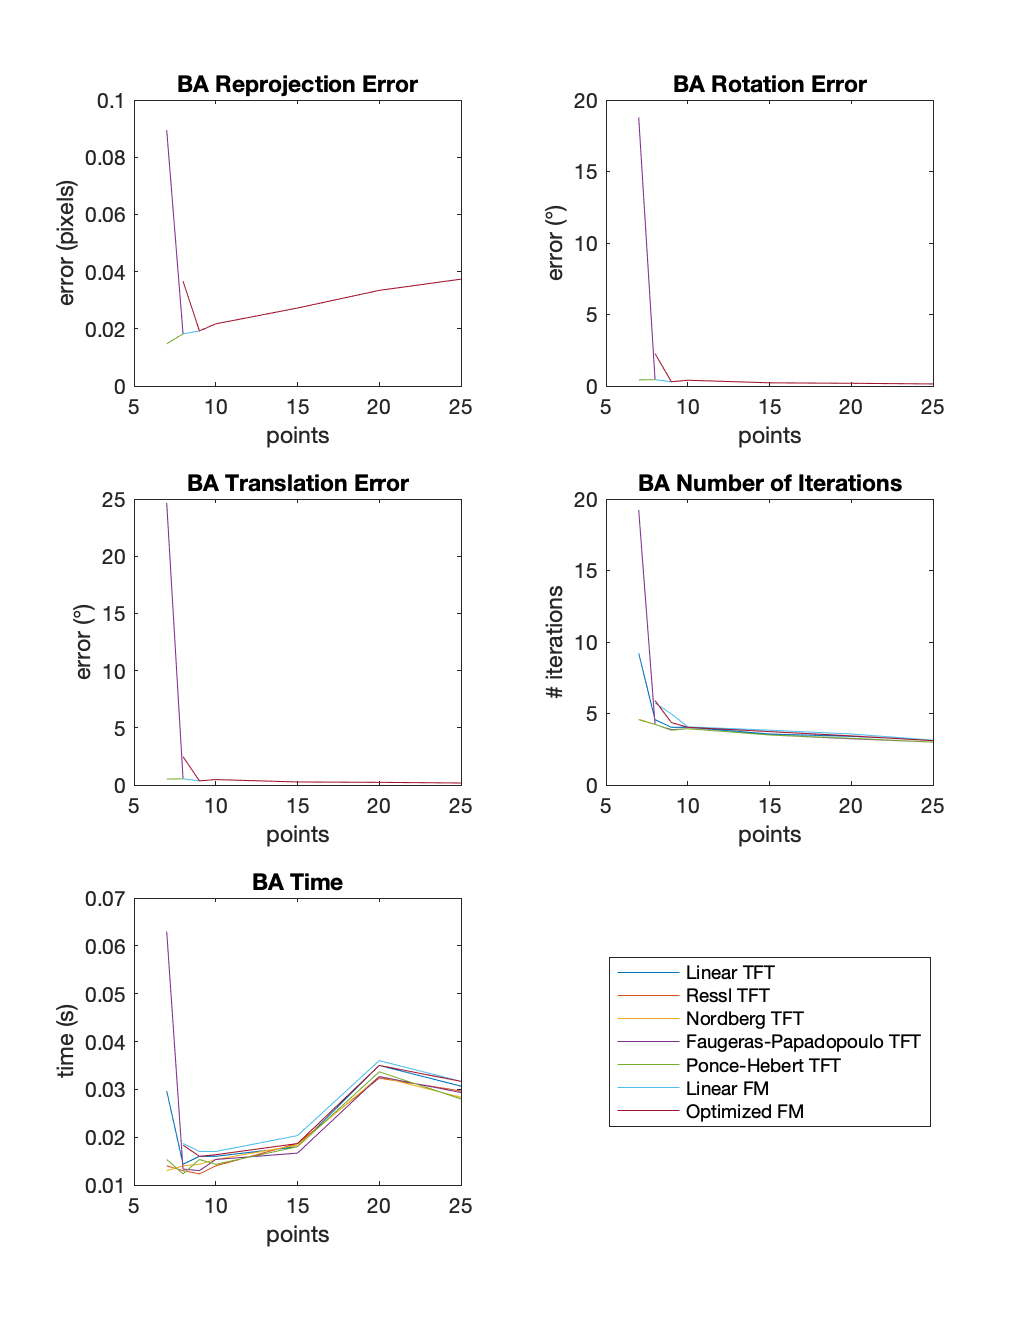
\includegraphics[width=1\textwidth]{Experiments/Synthetic/points/BApointsPlots.png}
	\caption[Synthetic Trial varying Number of Image Points with \acs{BA}]{Reprojection error (top-left), rotation error (top-right), translation error (mid-left), number of iterations (mid-right), computational time (bottom-left) after \acs{BA}; when varying the number of image points.}
	\label{fig:BAPointsPlot}
\end{figure}

\begin{figure}[p]
	\centering
	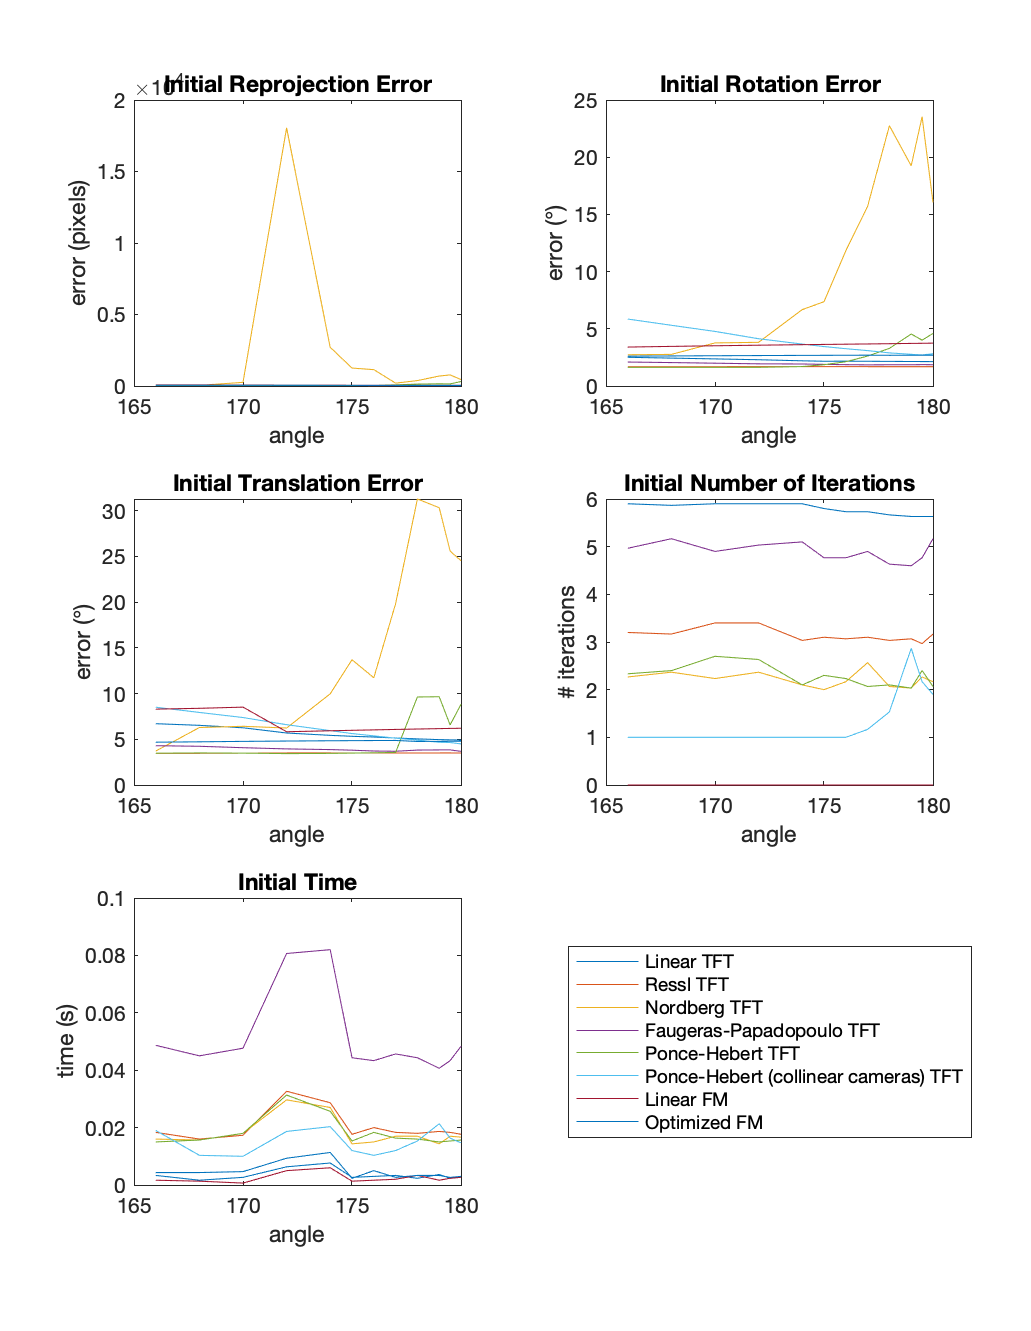
\includegraphics[width=1\textwidth]{Experiments/Synthetic/angle/INITanglePlots.png}
	\caption[Synthetic Trial varying Camera Centers Angle]{Initial reprojection error (top-left), rotation error (top-right), translation error (mid-left), number of iterations (mid-right), computational time (bottom-left); when varying the angle among the three camera centers.}
	\label{fig:initAnglePlot}
\end{figure}

\begin{figure}[p]
	\centering
	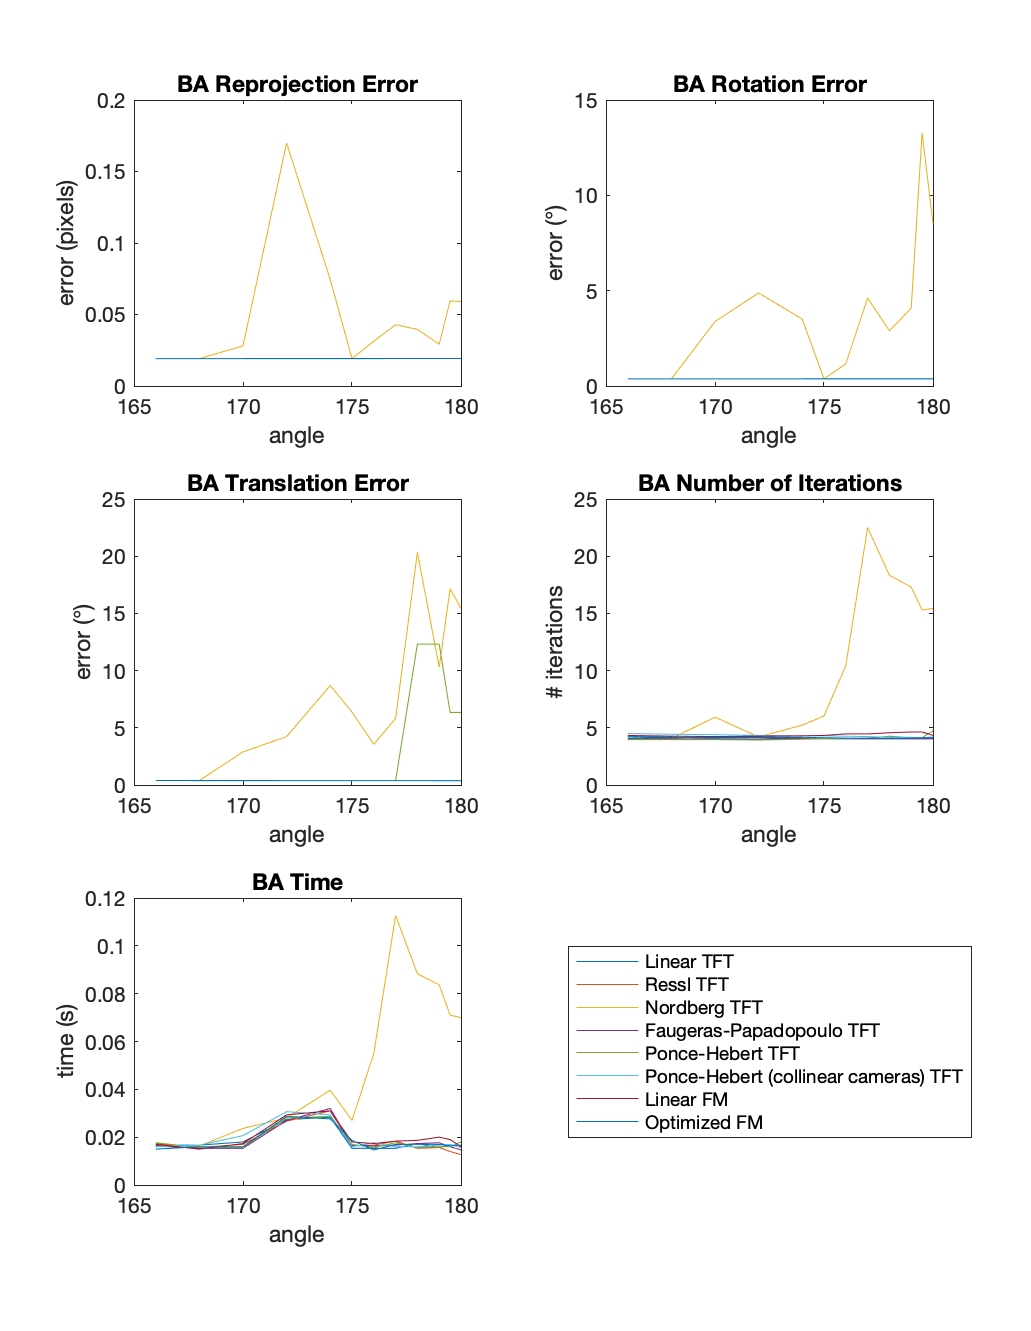
\includegraphics[width=1\textwidth]{Experiments/Synthetic/angle/BAanglePlots.png}
	\caption[Synthetic Trial varying Camera Centers Angle with \acs{BA}]{Reprojection error (top-left), rotation error (top-right), translation error (mid-left), number of iterations (mid-right), computational time (bottom-left) after \acs{BA}; when varying the angle among the three camera centers.}
	\label{fig:BAAnglePlot}
\end{figure}

\pagebreak

\subsection{Real Data}
In assessing the efficacy of these methods within real-world contexts, we opted to utilize scenes from the EPFL Dense Multi-View Stereo Dataset, presented in \cite{13-epfl-dataset}, provided by the CVLab at EPFL. \footnote{The EPFL Dense Multi-View Stereo Dataset, featuring the scenes utilized in our study, is readily accessible at the following location: \href{https://documents.epfl.ch/groups/c/cv/cvlab-unit/www/data/multiview/denseMVS.html}{https://documents.epfl.ch/groups/c/cv/cvlab-unit/www/data/multiview/denseMVS.html}.}\\

Table (\ref{tab:fountainInit}) and (\ref{tab:fountainBA}) show metrics before and after \acs{BA} with respect to the \textit{fountain-P11} set of images from the dataset.

\begin{figure}[h]
    \centering
    \subfigure[]{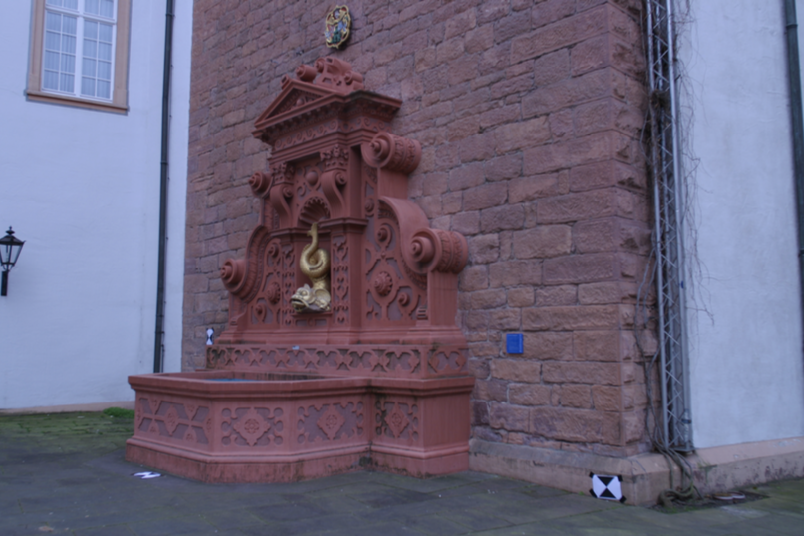
\includegraphics[width=0.30\textwidth]{Dataset/imgsReport/fountain1.png}} 
    \subfigure[]{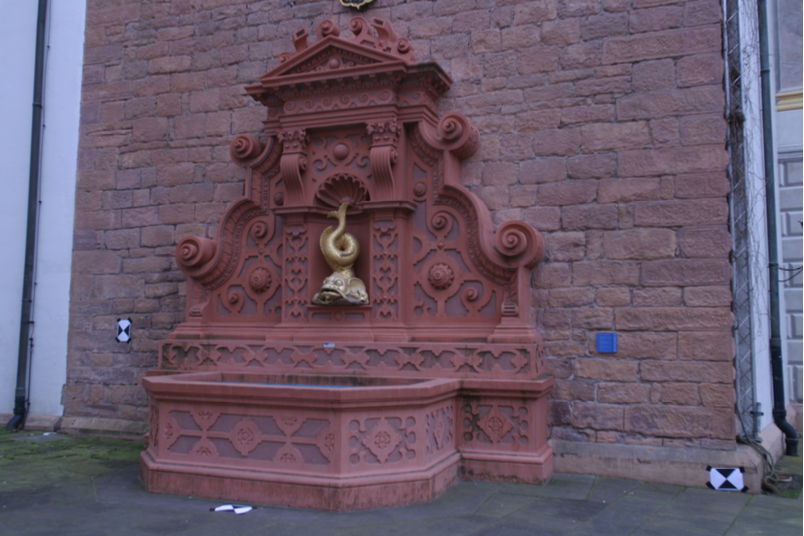
\includegraphics[width=0.30\textwidth]{Dataset/imgsReport/fountain2.png}} 
    \subfigure[]{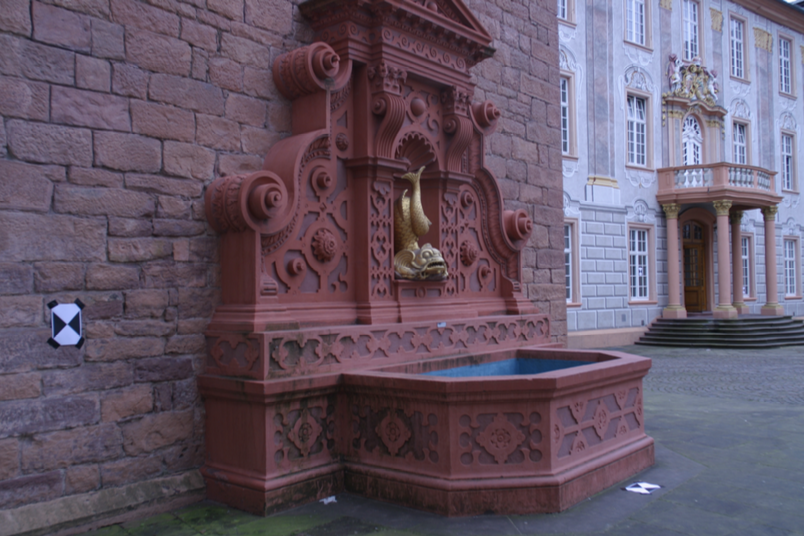
\includegraphics[width=0.30\textwidth]{Dataset/imgsReport/fountain3.png}}
    \caption[\textit{fountain-P11} Triplet]{Generic three-view triplet of images with respect to \textit{fountain-P11}. \cite{13-epfl-dataset}}
    \label{fig:fountainImage}
\end{figure}

\begin{table}[htbp]
  \centering
  \caption[\textit{fountain-P11} Initial Metrics]{Initial metrics with respect to the \textit{fountain-P11} set of images.}
  \label{tab:fountainInit}
  \begin{tabular}{|*{6}{c}|}
    \hline
     & repr. error (px) & R error ($^{\circ}$) & t error ($^{\circ}$) & \# iter. & time (s)\\
    \hline
    \acs{L-TFT} & 2.3953 & 0.1249 & 0.4048 & 0 & 0.0621 \\
    \acs{R-TFT} & 2.0474 & 0.1158 & 0.4003 & 2.8429 & 0.6400 \\
    \acs{N-TFT} & 2.1322 & 0.1334 & 0.4028 & 2.8000 & 0.6280 \\
    \acs{FP-TFT} & 2.3688 & 0.1187 & 0.4055 & 2.7714 & 0.6073 \\
    \acs{PH-TFT} & 2.0871 & 0.1167 & 0.4030 & 2.5857 & 0.5554 \\
    \acs{L-FM} & 1.9671 & 0.1149 & 0.3717 & 0 & 0.0273 \\
    \acs{O-FM} & 1.9530 & 0.1127 & 0.3658 & 4.9286 & 0.3209 \\
    \hline
  \end{tabular}
\end{table}

\begin{table}[htbp]
  \centering
  \caption[\textit{fountain-P11} Metrics with \acs{BA}]{Metrics after \acs{BA} with respect to the \textit{fountain-P11} set of images.}
  \label{tab:fountainBA}
  \begin{tabular}{|*{6}{c}|}
    \hline
     & repr. error (px) & R error ($^{\circ}$) & t error ($^{\circ}$) & \# iter. & time (s)\\
     \hline
    \acs{L-TFT} & 0.2814 & 0.0640 & 0.0743 & 3.8143 & 0.0743 \\
    \acs{R-TFT} & 0.2814 & 0.0640 & 0.0743 & 3.8286 & 0.0720 \\
    \acs{N-TFT} & 0.2814 & 0.0640 & 0.0743 & 3.8571 & 0.0716 \\
    \acs{FP-TFT} & 0.2814 & 0.0640 & 0.0743 & 3.8429 & 0.0723 \\
    \acs{PH-TFT} & 0.2814 & 0.0640 & 0.0743 & 3.8429 & 0.0743 \\
    \acs{L-FM} & 0.2814 & 0.0640 & 0.0743 & 3.7714 & 0.0816 \\
    \acs{O-FM} & 0.2814 & 0.0640 & 0.0743 & 3.8000 & 0.0784 \\
    \hline
  \end{tabular}
\end{table}

\pagebreak

Table (\ref{tab:HerzJesuInit}) and (\ref{tab:HerzJesuBA}) show metrics before and after \acs{BA} with respect to the \textit{Herz-Jesu-P8} set of images from the dataset.

\begin{figure}[h]
    \centering
    \subfigure[]{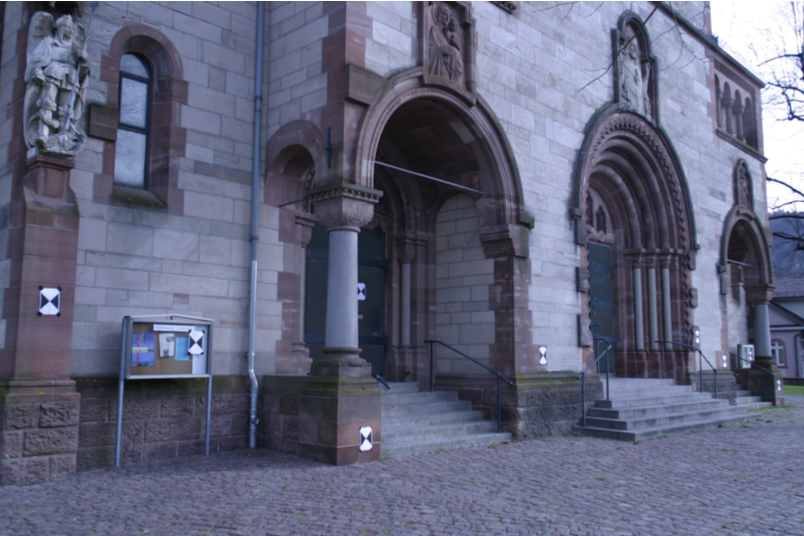
\includegraphics[width=0.30\textwidth]{Dataset/imgsReport/herzjesu1.png}} 
    \subfigure[]{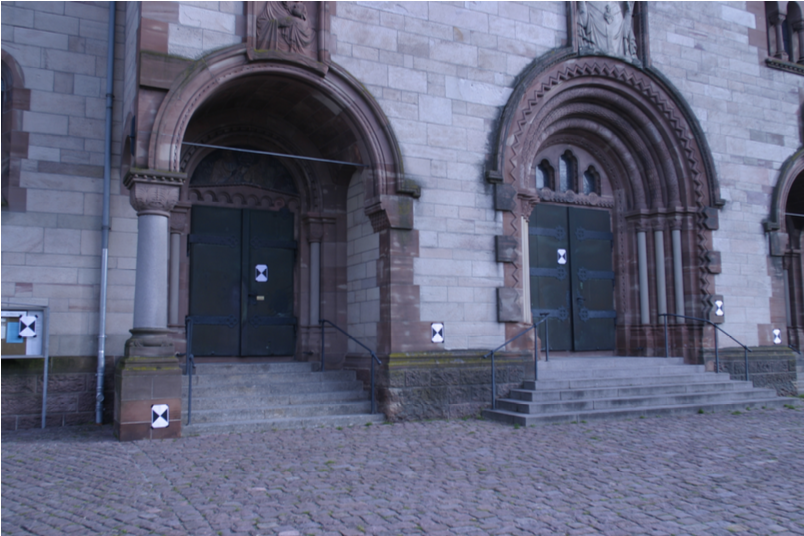
\includegraphics[width=0.30\textwidth]{Dataset/imgsReport/herzjesu2.png}} 
    \subfigure[]{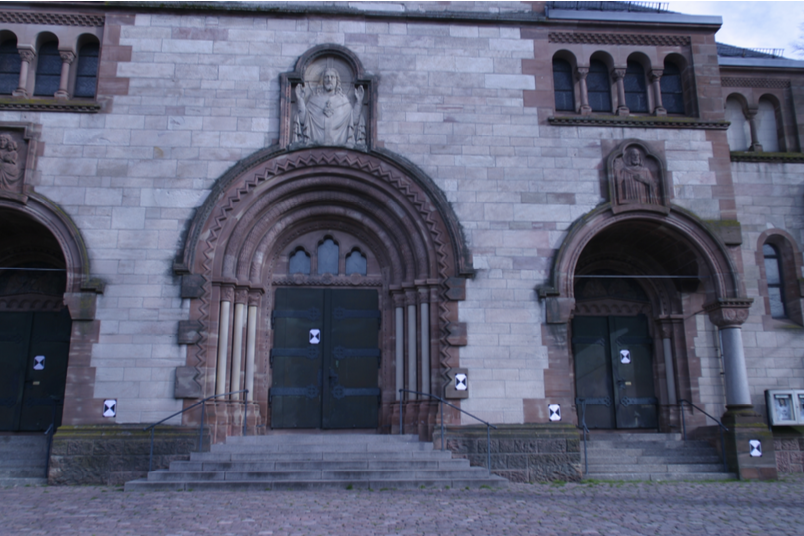
\includegraphics[width=0.30\textwidth]{Dataset/imgsReport/herzjesu3.png}}
    \caption[\textit{Herz-Jesu-P8} Triplet]{Generic three-view triplet of images with respect to \textit{Herz-Jesu-P8}. \cite{13-epfl-dataset}}
    \label{fig:herzjesuImage}
\end{figure}

\begin{table}[htbp]
  \centering
  \caption[\textit{Herz-Jesu-P8} Initial Metrics]{Initial metrics with respect to the \textit{Herz-Jesu-P8} set of images.}
  \label{tab:HerzJesuInit}
  \begin{tabular}{|*{6}{c}|}
    \hline
     & repr. error (px) & R error ($^{\circ}$) & t error ($^{\circ}$) & \# iter. & time (s)\\
    \hline
    \acs{L-TFT} & 4.8062 & 0.4589 & 0.8707 & 0 & 0.0506 \\
    \acs{R-TFT} & 3.4792 & 0.3966 & 0.6677 & 2.7800 & 0.4904 \\
    \acs{N-TFT} & 4.0656 & 0.5252 & 0.6917 & 2.6600 & 0.4816 \\
    \acs{FP-TFT} & 4.5006 & 0.4459 & 0.8324 & 3.4400 & 0.5452 \\
    \acs{PH-TFT} & 4.5293 & 0.4261 & 0.6682 & 2.3000 & 0.4116 \\
    \acs{L-FM} & 3.7624 & 0.4142 & 0.7725 & 0 & 0.0224 \\
    \acs{O-FM} & 3.6503 & 0.4196 & 0.7654 & 5.6600 & 0.2906 \\
    \hline
  \end{tabular}
\end{table}

\begin{table}[htbp]
  \centering
  \caption[\textit{Herz-Jesu-P8} Metrics with \acs{BA}]{Metrics after \acs{BA} with respect to the \textit{Herz-Jesu-P8} set of images.}
  \label{tab:HerzJesuBA}
  \begin{tabular}{|*{6}{c}|}
    \hline
     & repr. error (px) & R error ($^{\circ}$) & t error ($^{\circ}$) & \# iter. & time (s)\\
    \hline
    \acs{L-TFT} & 0.3719 & 0.0635 & 0.0682 & 4.0600 & 0.0792 \\
    \acs{R-TFT} & 0.3719 & 0.0635 & 0.0682 & 4.0000 & 0.0674 \\
    \acs{N-TFT} & 0.3719 & 0.0635 & 0.0682 & 4.0400 & 0.0690 \\
    \acs{FP-TFT} & 0.3719 & 0.0635 & 0.0682 & 4.0600 & 0.0680 \\
    \acs{PH-TFT} & 0.3719 & 0.0635 & 0.0682 & 4.0000 & 0.0664 \\
    \acs{L-FM} & 0.3719 & 0.0635 & 0.0682 & 4.0000 & 0.0718 \\
    \acs{O-FM} & 0.3719 & 0.0635 & 0.0682 & 4.0200 & 0.0724 \\
    \hline
  \end{tabular}
\end{table}

\pagebreak

Table (\ref{tab:entryInit}) and (\ref{tab:entryBA}) show metrics before and after \acs{BA} with respect to the \textit{entry-P10} set of images from the dataset.

\begin{figure}[h]
    \centering
    \subfigure[]{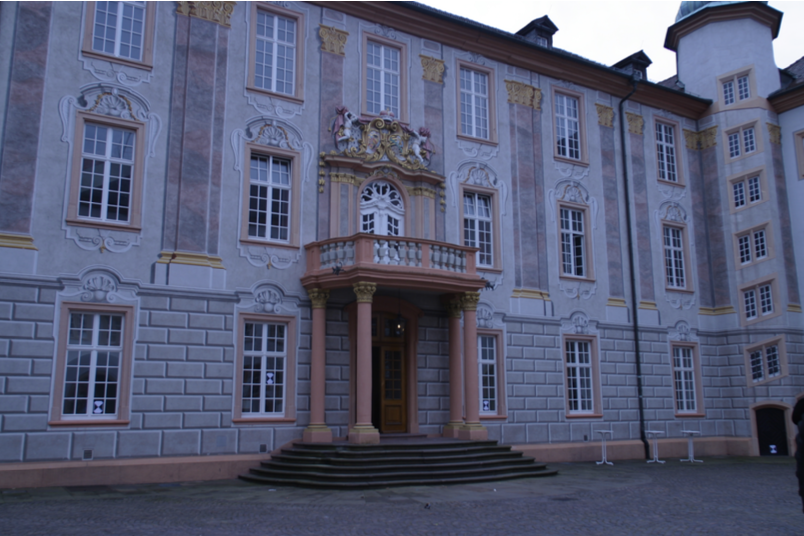
\includegraphics[width=0.30\textwidth]{Dataset/imgsReport/entry1.png}} 
    \subfigure[]{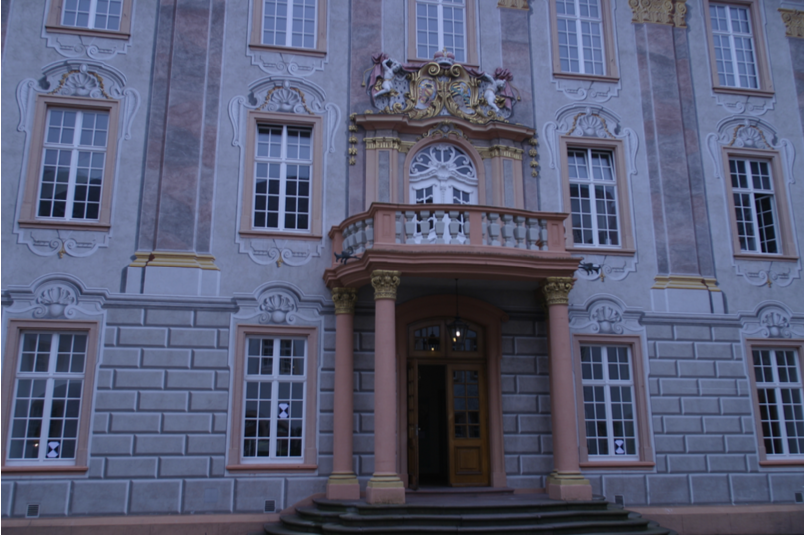
\includegraphics[width=0.30\textwidth]{Dataset/imgsReport/entry2.png}} 
    \subfigure[]{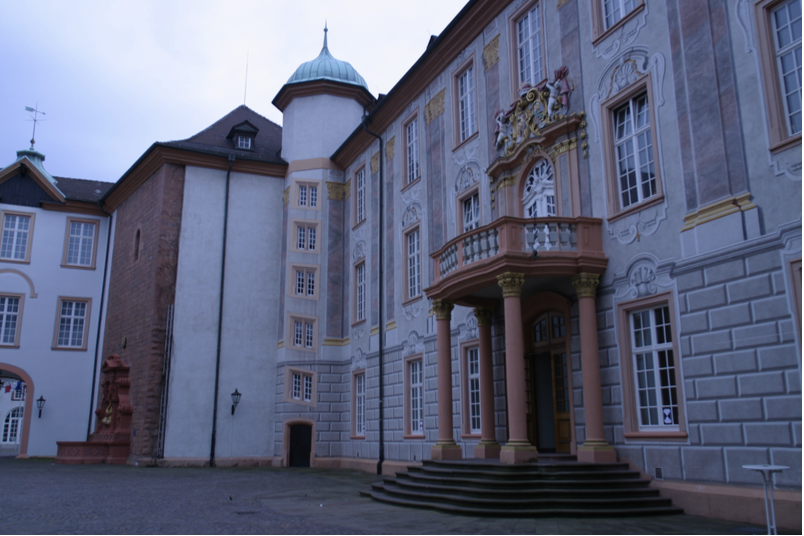
\includegraphics[width=0.30\textwidth]{Dataset/imgsReport/entry3.png}}
    \caption[\textit{entry-P10} Triplet]{Generic three-view triplet of images with respect to \textit{entry-P10}. \cite{13-epfl-dataset}}
    \label{fig:entryImage}
\end{figure}

\begin{table}[htbp]
  \centering
  \caption[\textit{entry-P10} Initial Metrics]{Initial metrics with respect to the \textit{entry-P10} set of images.}
  \label{tab:entryInit}
  \begin{tabular}{|*{6}{c}|}
    \hline
     & repr. error (px) & R error ($^{\circ}$) & t error ($^{\circ}$) & \# iter. & time (s)\\
    \hline
    \acs{L-TFT} & 3.8006 & 0.4144 & 0.8582 & 0 & 0.0572 \\
    \acs{R-TFT} & 3.1021 & 0.3872 & 0.6520 & 2.8200 & 0.5023 \\
    \acs{N-TFT} & 3.4590 & 0.4812 & 0.6833 & 2.7800 & 0.5144 \\
    \acs{FP-TFT} & 3.4480 & 0.4310 & 0.8246 & 3.5200 & 0.6340 \\
    \acs{PH-TFT} & 3.5078 & 0.4129 & 0.6619 & 2.4000 & 0.4389 \\
    \acs{L-FM} & 3.6451 & 0.4075 & 0.7103 & 0 & 0.0388 \\
    \acs{O-FM} & 3.6054 & 0.4018 & 0.7578 & 5.6800 & 0.3476 \\
    \hline
  \end{tabular}
\end{table}

\begin{table}[htbp]
  \centering
  \caption[\textit{entry-P10} Metrics with \acs{BA}]{Metrics after \acs{BA} with respect to the \textit{entry-P10} set of images.}
  \label{tab:entryBA}
  \begin{tabular}{|*{6}{c}|}
    \hline
     & repr. error (px) & R error ($^{\circ}$) & t error ($^{\circ}$) & \# iter. & time (s)\\
    \hline
    \acs{L-TFT} & 0.3479 & 0.0581 & 0.0634 & 4.0153 & 0.0811 \\
    \acs{R-TFT} & 0.3479 & 0.0581 & 0.0634 & 4.0242 & 0.0682 \\
    \acs{N-TFT} & 0.3479 & 0.0581 & 0.0634 & 4.0167 & 0.0708 \\
    \acs{FP-TFT} & 0.3479 & 0.0581 & 0.0634 & 4.0271 & 0.0714 \\
    \acs{PH-TFT} & 0.3479 & 0.0581 & 0.0634 & 4.0015 & 0.0679 \\
    \acs{L-FM} & 0.3479 & 0.0581 & 0.0634 & 3.9920 & 0.0734 \\
    \acs{O-FM} & 0.3479 & 0.0581 & 0.0634 & 4.0030 & 0.0751 \\
    \hline
  \end{tabular}
\end{table}

\pagebreak

Table (\ref{tab:castleInit}) and (\ref{tab:castleBA}) show metrics before and after \acs{BA} with respect to the \textit{castle-P19} set of images from the dataset.

\begin{figure}[h]
    \centering
    \subfigure[]{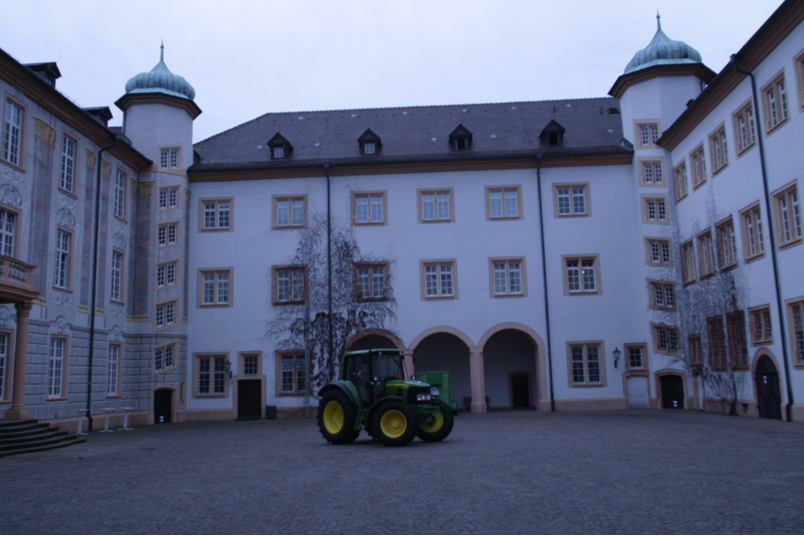
\includegraphics[width=0.30\textwidth]{Dataset/imgsReport/castle1.png}} 
    \subfigure[]{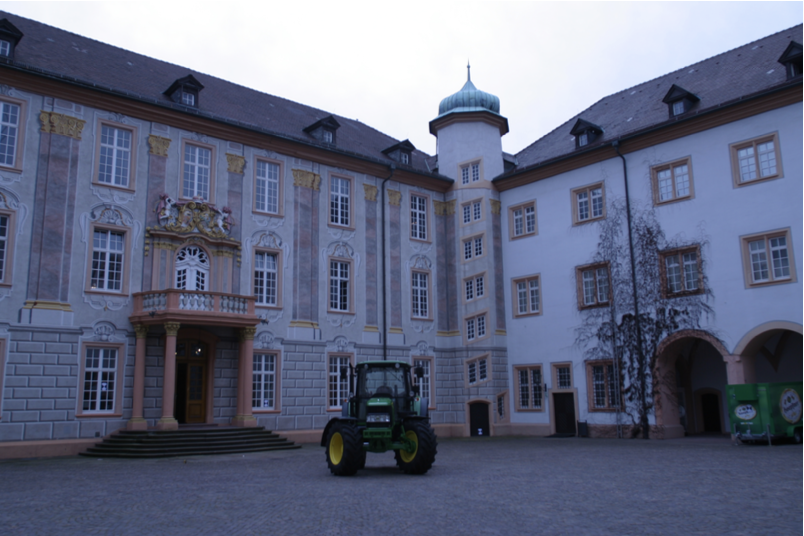
\includegraphics[width=0.30\textwidth]{Dataset/imgsReport/castle2.png}} 
    \subfigure[]{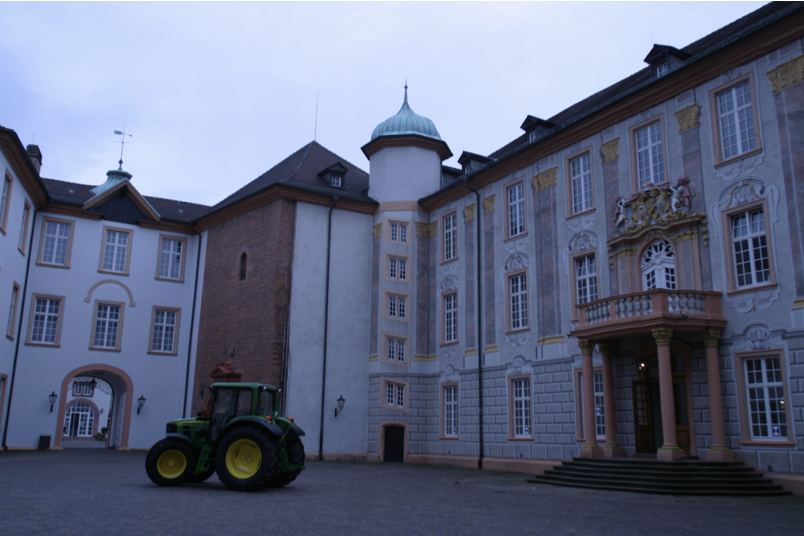
\includegraphics[width=0.30\textwidth]{Dataset/imgsReport/castle3.png}}
    \caption[\textit{castle-P19} Triplet]{Generic three-view triplet of images with respect to \textit{castle-P19}. \cite{13-epfl-dataset}}
    \label{fig:castleImage}
\end{figure}

\begin{table}[htbp]
  \centering
  \caption[\textit{castle-P19} Initial Metrics]{Initial metrics with respect to the \textit{castle-P19} set of images.}
  \label{tab:castleInit}
  \begin{tabular}{|*{6}{c}|}
    \hline
     & repr. error (px) & R error ($^{\circ}$) & t error ($^{\circ}$) & \# iter. & time (s)\\
    \hline
    \acs{L-TFT} & 3.7411 & 0.4235 & 0.8439 & 0 & 0.0614 \\
    \acs{R-TFT} & 2.8651 & 0.4147 & 0.6328 & 2.8400 & 0.5132 \\
    \acs{N-TFT} & 2.9337 & 0.4612 & 0.6740 & 2.7200 & 0.4922 \\
    \acs{FP-TFT} & 3.0164 & 0.4001 & 0.8125 & 3.5200 & 0.5478 \\
    \acs{PH-TFT} & 3.1450 & 0.4138 & 0.6574 & 2.4800 & 0.4227 \\
    \acs{L-FM} & 3.4568 & 0.3966 & 0.6913 & 0 & 0.0432 \\
    \acs{O-FM} & 3.5679 & 0.3810 & 0.7155 & 5.7800 & 0.4490 \\
    \hline
  \end{tabular}
\end{table}

\begin{table}[htbp]
  \centering
  \caption[\textit{castle-P19} Metrics with \acs{BA}]{Metrics after \acs{BA} with respect to the \textit{castle-P19} set of images.}
  \label{tab:castleBA}
  \begin{tabular}{|*{6}{c}|}
    \hline
     & repr. error (px) & R error ($^{\circ}$) & t error ($^{\circ}$) & \# iter. & time (s)\\
    \hline
    \acs{L-TFT} & 0.3583 & 0.0601 & 0.0657 & 4.0177 & 0.0827 \\
    \acs{R-TFT} & 0.3583 & 0.0601 & 0.0657 & 4.0211 & 0.0698 \\
    \acs{N-TFT} & 0.3583 & 0.0601 & 0.0657 & 4.0235 & 0.0716 \\
    \acs{FP-TFT} & 0.3583 & 0.0601 & 0.0657 & 4.0301 & 0.0721 \\
    \acs{PH-TFT} & 0.3583 & 0.0601 & 0.0657 & 4.0021 & 0.0684 \\
    \acs{L-FM} & 0.3583 & 0.0601 & 0.0657 & 3.9974 & 0.0733 \\
    \acs{O-FM} & 0.3583 & 0.0601 & 0.0657 & 4.0081 & 0.0742 \\
    \hline
  \end{tabular}
\end{table}

Unsurprisingly, considering the results obtained with the synthetic experiments, the \acs{BA} has a major influence on the performances with respect to the different mathematical structures considered (\eg, \acs{FM}, \acs{TFT}, parametrizations of the \acs{TFT}).

In fact, regardless of the pose estimation technique considered, all errors (post-\acs{BA}) converge to a fixed value, which is significantly lower than all the corresponding error values computed with the different parametrizations.\\

\section{Conclusions}\label{sec:conclusions}
In our study, we explored different methods for estimating the trifocal tensor and figuring out the positions of three separate views. After thorough testing, we found that even though the trifocal tensor is a valid method, it doesn't offer enough benefits over using fundamental matrices from pairs of views to make it the better choice.\\

Our results highlight the practical benefits of simplicity and efficiency. We recommend focusing on pairwise constraints using fundamental matrices and then refining the results with bundle adjustment techniques. It's important to mention that bundle adjustment consistently reduces errors significantly. In this approach, the first step is to establish pairwise constraints to determine the relative scales of translations, using image triplets mainly for this purpose.

\subsection{Future Work}
Another interesting direction for future analysis is to see if using the trifocal tensor gives better results when working with more than three views (\ie, \( n > 3 \)). In such multi-view stereo setups, the way image pairs and triplets are combined will likely have a big impact on the overall effectiveness.\\

Our work also showed something important about bundle adjustment optimisation. We discovered that even if we start the process from very different points, it can still end up at a good solution. This means there might be a bigger area where the optimisation works well, and we plan to look into this more in future studies.


%\appendix
%\section{Supplementary Material}

{\small
\bibliographystyle{ieee}
\bibliography{egbib}
}

\end{document}
